\documentclass[paper=A4,%
parskip=half,
%BCOR=1cm % Mehr Platz am Rand fürs Binden!
draft=false,
abstracton
%firstfoot=false
]{scrartcl}

\addtokomafont{sectioning}{\rmfamily}
\setkomafont{title}{\normalfont\scshape}
\DeclareOldFontCommand{\bf}{\normalfont\bfseries}{\mathbf}
%So that headings are also in serif


% Settings for optimal screen viewing (my laptop screen)
% \documentclass[twocolumn]{article}
% \usepackage[top=0.1in, bottom=0.1in, left=0.3in, right=0.3in, paperwidth=9in, paperheight=4in]{geometry}

%!TEX root = ./master.tex
%%% PACKAGES

% XeLaTeX
\usepackage{xltxtra}

% Inernational
\usepackage[ngerman, english]{babel}

% math stuff
\usepackage{
  amsmath,
  amssymb,
  amsthm,
  mathtools,
  latexsym
}

%so that amsmath plays nice with parskip
% \makeatletter
% \def\thm@space@setup{%
%   \thm@preskip=\parskip \thm@postskip=0pt
% }
% \makeatother

% more arrows
\usepackage{stmaryrd} % for mapsfrom
\usepackage{extarrows} % for xlongrightarrow

% more symbols
\usepackage{upgreek} % upright greek letters

% more flexible enumerations
\usepackage{enumitem}
\setlist[enumerate]{labelwidth=!,wide,labelindent=0pt,itemsep=0pt,label=(\roman*)}
\newcommand{\huyitem}{\normalfont \rmfamily \item \normalfont \itshape}

% for commutative diagrams
\usepackage{tikz-cd}
\usetikzlibrary{babel} % otherwise babel fucks up tikzcd

% aesthetics
%\usepackage{subdepth} % consistent use of simultaneous subscripts and supscripts
\usepackage{ellipsis} % right ellipsis when using \dots, include after xltxtra
\usepackage{microtype} % better everything

% typographic settings
%\usepackage[margin=1.3in]{geometry}
% \usepackage{geometry}
% \usepackage{calc}
% \newcommand{\alphabet}{%
%   abcdefghijklmnopqrstuvwxyz%
% }
% \newlength{\textW}
% \setlength{\textW}{\widthof{\alphabet}* \real{2.5}}
% \geometry{textwidth=\textW,}
%\usepackage[dmyyyy]{datetime}
%\renewcommand{\dateseparator}{.}

% Latin modern font choice
\usepackage{lmodern}

% Libertinus font choice, copied from project's Github
% \usepackage{unicode-math}
% \setmainfont{Libertinus Serif}
% \setsansfont{Libertinus Sans}
% \setmathfont[AutoFakeBold]{Libertinus Math}
% \setmathfont[range={\mathcal, \mathscr}]{xits-math.otf}
% \setmathfont[range={}]{Libertinus Math}

% paragraph settings
%\setlength{\parindent}{0cm} % no paragraph indentation
%\setlength{\parskip}{0.6em} % wider paragraph spacing

%\usepackage{parskip}

% Hyperlinks in references
\usepackage[bookmarks, colorlinks, breaklinks]{hyperref}
\usepackage{cleveref} % \cref, \Cref

\usepackage{multirow}  % for `\multirow` macro

\usepackage{mycommands} 

% Bibliography
\usepackage[backend=biber, style=alphabetic, isbn=false, url=true, doi=false, maxbibnames=99]{biblatex}
\renewbibmacro{in:}{}
\DefineBibliographyStrings{english}{% no p. or pp. before pages
  page             = {},
  pages            = {},
}
% to remove quotes
\DeclareFieldFormat[article,inbook,incollection,inproceedings,patent,thesis,unpublished]{citetitle}{#1}
\DeclareFieldFormat[article,inbook,incollection,inproceedings,patent,thesis,unpublished]{title}{#1}

\addbibresource{masterarbeit-bib.bib}
\setlength\bibitemsep{\parskip}
% maybe collect bib settings into separate file... another file to track...

%%% TEXT SETTINGS
\definecolor{darkgreen}{rgb}{0.0, 0.2, 0.13}
% link colors
\hypersetup{linkcolor=blue,citecolor=darkgreen,filecolor=black,urlcolor=cyan}

% theorems
\newtheorem{theorem}{Theorem}[section]
\newtheorem{proposition}[theorem]{Proposition}
\newtheorem{lemma}[theorem]{Lemma}
\newtheorem{corollary}[theorem]{Corollary}
\newtheorem{conjecture}[theorem]{Conjecture}

\theoremstyle{definition}
\newtheorem{definition}[theorem]{Definition}
\newtheorem{remark}[theorem]{Remark}
\newtheorem{example}[theorem]{Example}
\newtheorem{computation}[theorem]{Computation}
\newtheorem{construction}[theorem]{Construction}
\newtheorem{claim}{Claim}[theorem]

\newenvironment{subproof}[1][\proofname]{%
  \renewcommand{\qedsymbol}{$\blacksquare$}%
  \begin{proof}[#1]%
}{%
  \end{proof}%
}



% numbering settings
%\renewcommand{\thesection}{\arabic{section}.}
%\renewcommand{\thesubsection}{\arabic{section}.\arabic{subsection}.}
%\renewcommand{\thesubsubsection}{\arabic{section}.\arabic{subsection}.\arabic{subsubsection}.}
%\renewcommand{\thetheorem}{\arabic{section}.\arabic{theorem}}
%\renewcommand{\theequation}{\arabic{section}.\arabic{equation}}
\usepackage{chngcntr}
%\counterwithout{equation}{section} % undo numbering system provided by phstyle.cls
\counterwithin{equation}{section}
\crefformat{equation}{\textup{#2(#1)#3}}
%\renewcommand{\ref}{\cref}
% hypenation
\hyphenation{mo-no-dro-my}

%%% PAST GOOD IDEAS

% Abbreviations
\newcommand{\ie}{i.e.\ }
\newcommand{\eg}{e.g.\ }
\newcommand{\cf}{cf.\ }

\newcommand{\isom}{\simeq}
\newcommand{\mrm}{\mathrm}
\DeclareMathOperator{\im}{im}
\newcommand{\wtilde}{\widetilde}
\DeclareMathOperator{\characteristic}{char}
\DeclareMathOperator{\codim}{codim}
%\DeclareMathOperator{\deg}{deg}
%\DeclareMathOperator{\ker}{ker}
%\newcommand{\pr}{\mathrm{pr}}

% Symbols
\newcommand{\leer}{\varnothing} % preferred symbol for the empty set
%\newcommand{\singleton}{\{\mathrm{pt}\}} % may also consider ``{*}''

% Accents
%\newcommand{\closure}[2][3]{ % closure for bigger symblos
%  {}\mkern#1mu\overline{\mkern-#1mu#2}}

% The perfect :=
% \newcommand*{\defeq}{\mathrel{\rlap{
%  \raisebox{0.3ex}{$\m@th\cdot$}}
%  \raisebox{-0.3ex}{$\m@th\cdot$}}
% =}

% Arrows
% \newcommand{\isom}{\xrightarrow{\sim}}

% Brackets
% \newcommand{\dblbrack}[1]{\left[\!\left[#1\right]\!\right]}
 \newcommand{\gen}[1]{\left\langle #1 \right\rangle}
% \newcommand{\floor}[1]{\left \lfloor #1 \right\rfloor}
% \newcommand{\abs}[1]{|#1|}

% Diagrams and Matrices
%\newcommand{\ses}[6]{ % short exact sequence!
%  \begin{tikzcd}[ampersand replacement=\&]
%  #1 \arrow{r} \& {#2} \arrow{r}{#5} \& {#3} \arrow{r}{#6} \& {#4} \arrow{r} \& #1
%  \end{tikzcd}
%}
%\newcommand{\smatrix}[1]{\left(\begin{smallmatrix}#1\end{smallmatrix}\right)} % small matrix
\newcommand{\GGr}{\mathbb G \mathrm r}

\newcommand{\schemeofsurfaces}{\abs{\mc{O}(d)}}
\newcommand{\schemeofquartics}{\abs{\mc{O}(4)}}
\newcommand{\schemeofsections}[1]{\abs{\mc{O}(#1)}}
\newcommand{\divides}{\mid}
\DeclarePairedDelimiter\ceil{\lceil}{\rceil}
\DeclarePairedDelimiter\floor{\lfloor}{\rfloor}

\setcounter{tocdepth}{1}

% %Name of the author of the thesis 
% \authornew{Orlando Marigliano}
% %Date of birth of the Author
% \geburtsdatum{5th August 1994}
% %Place of Birth
% \geburtsort{Rome, Italy}
% %Date of submission of the thesis
% \date{10th January 2018}
% %Name of the Advisor
% % z.B.: Prof. Dr. Peter Koepke
% \betreuer{Advisor: Prof.\ Daniel Huybrechts}
% %Name of the Insitute of the advisor
% \zweitgutachter{Second Advisor: Dr.\ Andrey Soldatenkov}
% %name of the second advisor of the thesis
% %z.B.: Mathematisches Institut
% \institut{Mathematical Institute}
% %Title of the thesis 
% \title{Verlinde Bundles of Families of Hypersurfaces}
% %Do not change!
% \ausarbeitungstyp{Master's Thesis  Mathematics}

\title{Verlinde bundles of families of hypersurfaces and their jumping lines}
\author{Orlando Marigliano}

\begin{document}
%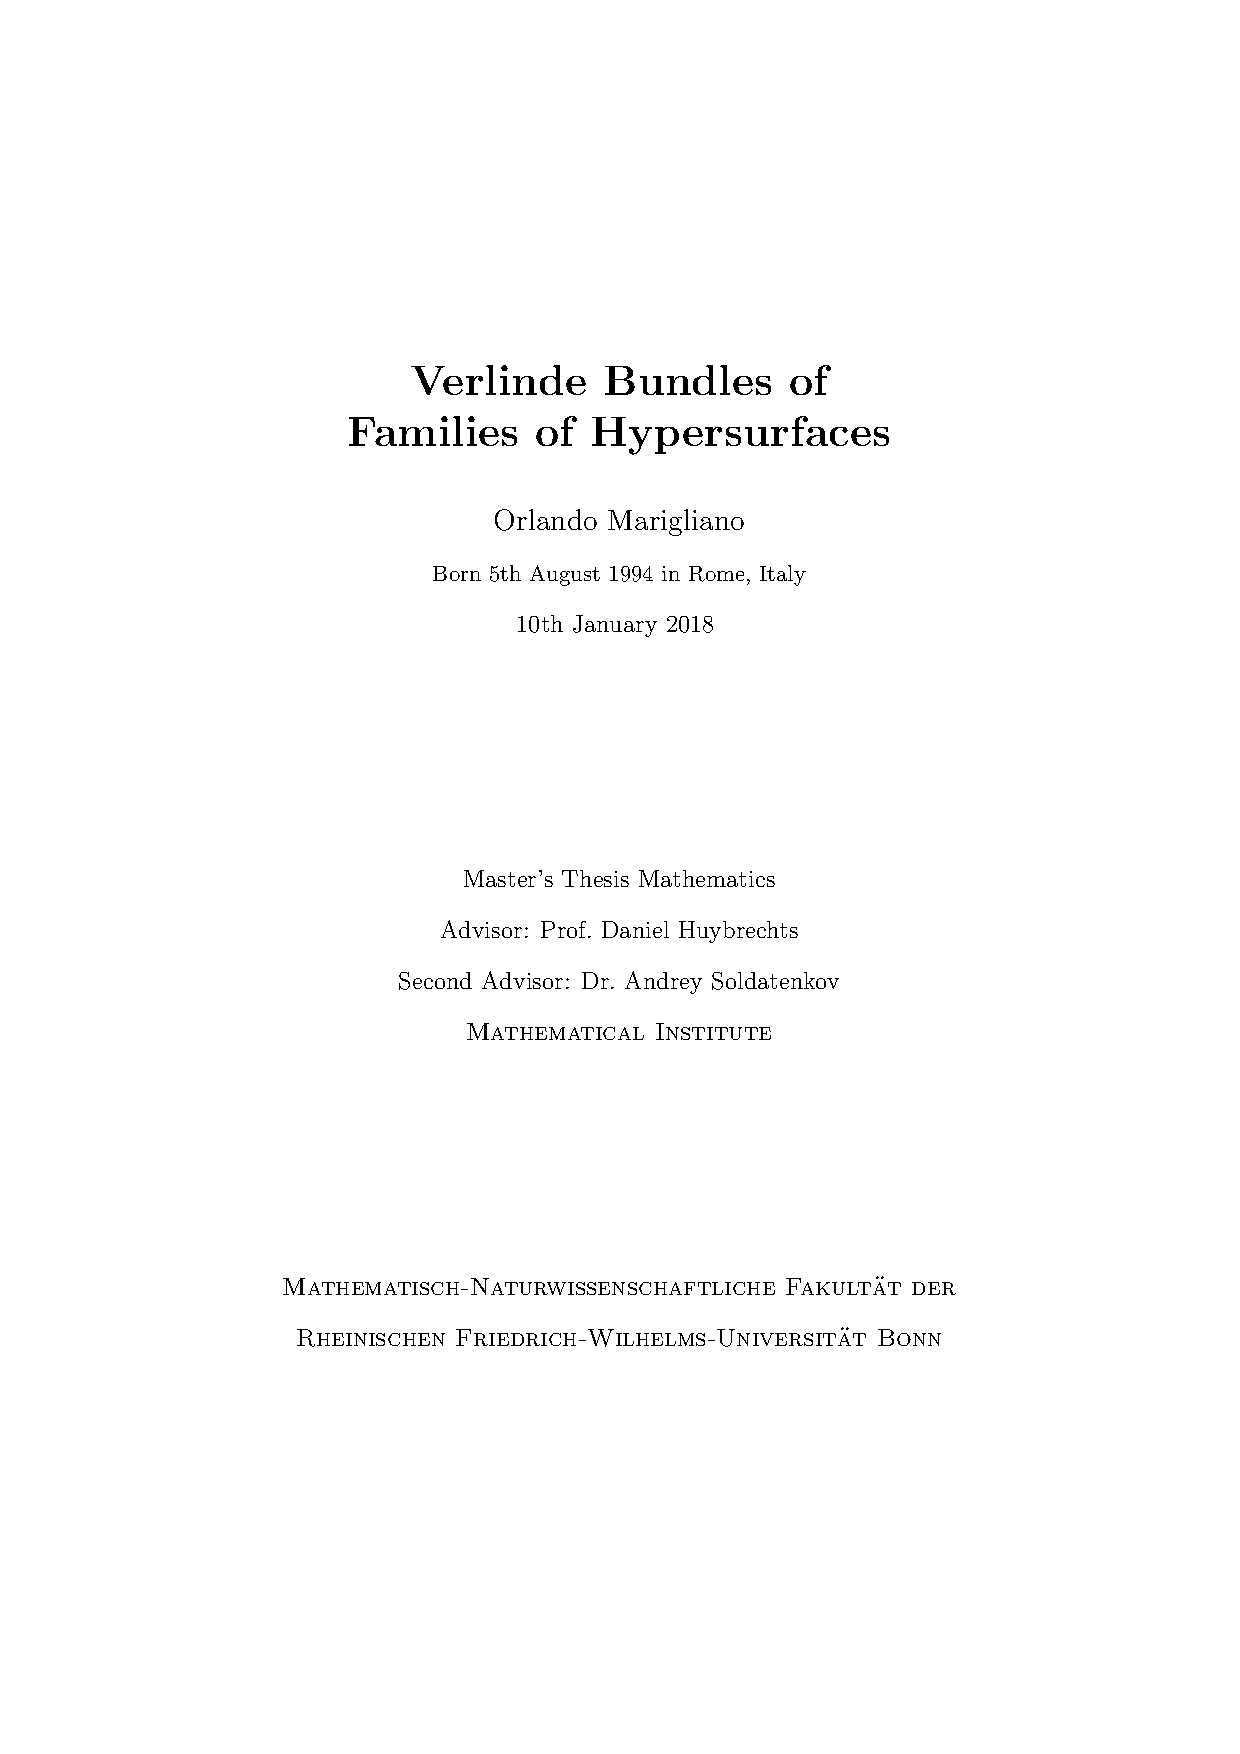
\includepdf[pages={-}]{myThesis}
\maketitle
\begin{abstract}
	\noindent Verlinde bundles are vector bundles $V_k$ arising as the direct image $\pi_*(\mc L^{\otimes k})$ of polarizations of a proper family of schemes $\pi\colon \mathfrak X \to S$. We study the splitting behavior of Verlinde bundles in the case where $\pi$ is the universal family $\mathfrak X \to \schemeofsurfaces$ of hypersurfaces of degree $d$ in $\schemeofsurfaces$ and calculate the cohomology class of the locus of jumping lines of the Verlinde bundles
	$V_{d+1}$ in the cases $n=2,3$.  
\end{abstract}
%\tableofcontents
%Bisherige Kapitel
%%!TEX root = ./master.tex
\section{Introduction}

Let $\pi\from X\to S$ be a flat proper morphism of schemes, $\mc{L}$ an ample line bundle on $X$. The line bundle $\mc{L}$ and its powers $\mc{L}^{\otimes k}$ give information about how to embed the members $X_s$ of the family $\pi$ into the projective space, and how these embeddings vary along $S$. To better understand the family $\pi$, one can study the pushforwards
$V_k\coloneqq \pi_*(\mc{L}^{\otimes k})$, for $k\geq 1$. In good situations, $V_k$ is a vector bundle on $S$ and we have $V_k|_s = H^0(X_s, \mc{L}^{\otimes k})$ for $s\in S$. The $V_k$ are then called the \emph{Verlinde bundles} of the family $\pi$.

This thesis examines the situation where $\pi$ is the universal family of hypersurfaces of degree $d$ in $\PP^n$, where $n>1$. The Verlinde bundles are then defined on $\schemeofsurfaces$, which is a projective space of dimension $\binom{d+n}{n} - 1$.

We focus on the restriction $V_k|_T$ of the Verlinde bundles to lines $T\subset \schemeofsurfaces$, asking which isomorphism types of bundles on $\PP^1$ can occur as some such restriction, and how these types depend on $T$. For this, we study the associated subsets of the Grassmannian on lines in $\schemeofsurfaces$ consisting of lines $T$ such that $V_k|_T$ has a fixed isomorphism type. Lastly, we investigate some global statements about $V_k$, sometimes using its restriction to lines.

\subsection{Notation and conventions}
Throughout, $k$ will denote an algebraically closed field, but we omit it from most notation. The letter $k$ will also denote a natural number.

For natural numbers $d$ and $n$, we write $I_d$ for a tuple of non-negative integers of the form $(i_0,\dotsc,i_n)$ with
$\sum i_j = d$. Thus for example a tuple ranging over the $I_d$ will have $\binom{n+d}{n}$ entries.

We fix names for the homogeneous coordinates of various projective spaces: for the coordinates of $\PP^1$ we write $s$ and $t$, for $\PP^n$ we write $x_i$, and for the coordinates of $\schemeofsurfaces$ we take $\alpha_{I_d}$, where we think of $\alpha_{I_d}$ as corresponding to $x^{I_d}\coloneqq \prod_{i} x_i^{(I_d)_i}$.

For a fiber product $X \xleftarrow{p} X\times Y\xrightarrow{q} Y$ and sheaves $\mc{F}$ and $\mc{G}$ on $X$ resp.\ $Y$, we write $\mc{F}\boxtimes \mc{G}\coloneqq \pullb{p} \mc{F} \otimes \pullb{q} \mc{G}$.

\subsection{Aknowledgements}
I would like to take the opportunity to thank my advisor Daniel Huybrechts for his assistance, guidance, and mentorship during the writing of this thesis. I also thank my family for their financial and moral support throughout my studies, and my colleagues and friends at the Student Lounge for having made me look forward to every day of thesis work.
%%!TEX root = ./master.tex
\section{Introduction}

% \subsection{Notation and conventions}
% Throughout, $k$ will denote an algebraically closed field, but we omit it from most notation. The letter $k$ will also denote a natural number.

% For natural numbers $d$ and $n$, we write $I_d$ for a tuple of non-negative integers of the form $(i_0,\dotsc,i_n)$ with
% $\sum i_j = d$. Thus for example a tuple ranging over the $I_d$ will have $\binom{n+d}{n}$ entries.

% We fix names for the homogeneous coordinates of various projective spaces: for the coordinates of $\PP^1$ we write $s$ and $t$, for $\PP^n$ we write $x_i$, and for the coordinates of $\schemeofsurfaces$ we take $\alpha_{I_d}$, where we think of $\alpha_{I_d}$ as corresponding to $x^{I_d}\coloneqq \prod_{i} x_i^{(I_d)_i}$.

% For a fiber product $X \xleftarrow{p} X\times Y\xrightarrow{q} Y$ and sheaves $\mc{F}$ and $\mc{G}$ on $X$ resp.\ $Y$, we write $\mc{F}\boxtimes \mc{G}\coloneqq \pullb{p} \mc{F} \otimes \pullb{q} \mc{G}$.

\subsection{Aknowledgement}
This work is a condensed version of my Master's thesis, supervised by Daniel Huybrechts. I would like to take the opportunity to thank him for his mentorship during the writing of the thesis, as well as for his help during the preparation of this article.
%%!TEX root = ./master.tex
\section{Universal Families of Extensions}

Let $X$ and $S$ be Noetherian schemes over a field $k$. Let $f \from X \to S$ be a flat, projective morphism, and let $\mc{F}$ and $\mc{G}$ be coherent $\mc{O}_X$-modules, flat over $\mc{O}_S$.

Recall that an element $\xi \in \Ext^1_{X}(\mc{F},\mc{G})$ corresponds to an equivalence class of short exact sequences, or \emph{extensions}, of the form
\[
	\ses{\mc{G}}{\mc{E}}{\mc{F}},
\]
where two such sequences are equivalent if there exists an isomorphism between them that induces the identity on $\mc{F}$ and $\mc{G}$. The set of these equivalence classes can be given the structure of an $H^0(S,\mc{O}_S)$-module, see for example \cite[{}3.4]{weibel-homological-algebra}. This correspondence is functorial in both arguments, and preserves the $H^0(S, \mc{O}_S)$-module structure.

Explicitely, the sum of two elements of $\Ext^1$ corresponds to the Baer sum of the associated extensions, while the multiplication of an extension
as above by a scalar $a\in H^0(S,\mc{O}_S)$ is given by the pullback sequence along the map $\mc{F}\xto{a}\mc{F}$.

In this section, we ask when it is possible to construct an $S$-scheme $V$ and a universal extension on $X\times_S V$. This is found to be true for $\mc{F},\mc{G}$ locally free and $S=\Spec(k)$. For the more general situation, the article \cite{lange-universal-extensions} turns to the moduli problem of classifying relative extensions of sheaves and applies it to the global situation.
%The next proposition shows there exists a $k$-scheme $V$ that parametrizes the points of $\Ext^{1}_X(\mc{F},\mc{G})$.

\begin{remark} \label{small-spectral-sequence}
Let $\phi \from X_1 \to X_2$ be a morphism of schemes, let $\mc{F}_1$ and $\mc{F}_2$ be $\mc{O}_{X_1}$-modules. The Grothendieck spectral sequence \cite[Theorem~23.3.5]{vakil-algebraic-geometry} specializes to the Leray spectral sequence
$E_2^{p,q}=H^p(X_2,R^q \phi_*\mc{F}_1) \Rightarrow H^{p+q}(X_1,\mc{F}_1)$
%\cite[Theorem~23.4.5]{vakil-algebraic-geometry}
and the local-to-global $\Ext$ spectral sequence
$E_2^{p,q}=H^p(X_1,\EXT^q(\mc{F}_1,\mc{F}_2)) \Rightarrow \Ext^{p+q}(\mc{F}_1,\mc{F}_2)$.
The first few terms of the associated exact sequences in lower degrees are 
\begin{equation}
	0
	\to H^1(X_2,\pushf \phi \mc{F}_1)
	\to H^1(X_1,\mc{F}_1)
	\to H^0(X_2, R^1 \pushf \phi \mc{F}_1) \label{leray-es}
\end{equation}
and
\begin{equation}
	0
	\to H^1(X_2,\HOM(\mc{F}_1,\mc{F}_2))
	\to \Ext^1(\mc{F}_1,\mc{F}_2)
	\to H^0(X_2,\EXT^1(\mc{F}_1,\mc{F}_2)). \label{ext-es}
\end{equation}
\end{remark}

\begin{proposition} \label{cor:universal-extension}
Let $\mc{F}$ and $\mc{G}$ be locally free, and let $V \coloneqq \VV(\Ext^1_X(\mc{F},\mc{G})\dual)$. There exists an extension
	\[
		\xi_{\mathrm{univ}} \colon \quad \ses{\pullb{\pr_1}\mc{G}}{\mc{E}}{\pullb{\pr_1}\mc{F}}
	\]
over $X\times_k V$
such that for all Noetherian $k$-schemes $Y$, the map
$$\Mor_{k}(Y,V)\to\Ext^1_{X_Y}(\mc{F}_Y,\mc{G}_Y)$$ defined by
$\alpha \mapsto \pullb{(\id_X\times \alpha)} \xi_{\mathrm{univ}}$
is a bijection, functorial in $Y$.
In particular, pulling back $\xi_{\mathrm{univ}}$ gives a bijection $\Mor_{k}(\Spec(k),V)\xto{\sim} \Ext^1_{X}(\mc{F},\mc{G})$.
\end{proposition}

\begin{proof}
We denote the maps in the cartesian square $Y\times X$ as follows:
\[
	\cartesiansquare{Y\times X}{\pr_1}{Y} {\pr_2}{s_2} {X}{s_1}{k}
\]
We find functorial isomorphisms
\begin{align}
\Mor_{k}(Y,V)
% & \simeq \Hom_{\text{k-mod}}(\Ext^1_X(\mc{F},\mc{G})\dual,A) \label{ext-isom-univprop}\\
%\simeq & A \otimes_k \Ext^1_{X}(\mc{F},\mc{G}).
& \simeq H^0(\mc{O}_Y \otimes \Ext^1(\mc{F},\mc{G})) \label{isom-univprop} \\
& \simeq H^0(s_{2}^* H^1(\HOM(\mc{F},\mc{G}))) \label{isom-ext-ss} \\
& \simeq H^0(R^1 \pr_{2,*}(\pr_1^* \HOM(\mc{G},\mc{F}))) \label{isom-cbc} \\
& \simeq H^0(R^1 \pr_{2,*}(\HOM(\mc{F}_Y,\mc{G}_Y))) \label{isom-locfree}\\
& \simeq H^1(\HOM(\mc{G}_Y,\mc{F}_Y)) \label{isom-leray-ss-via-cbc}\\
& \simeq \Ext^1_{X_Y}(\mc{F}_Y,\mc{G}_Y) \label{isom-ext-ss-two}.
\end{align}
The required universal extension is then the image of $\id\in\Mor_{k}(V,V)$ in $\Ext^1_{X_Y}(\mc{F}_Y,\mc{G}_Y)$.

The isomorphism \cref{isom-univprop} comes from the universal property of $\VV(\Ext^1_X(\mc{F},\mc{G})\dual)$. The isomorphisms \cref{isom-ext-ss} and \cref{isom-ext-ss-two} come from the sequence \cref{ext-es}, whose third term is zero since $\mc{F}$ and $\mc{G}$ are locally free. We have \cref{isom-cbc} by the Cohomology and Base Change Theorem \cite[{}28.1.6]{vakil-algebraic-geometry}, and \cref{isom-locfree} since $\mc{F}$ and $\mc{G}$ are locally free. For the isomorphism \cref{isom-leray-ss-via-cbc}, we use the sequence \cref{leray-es}, whose third term is found to be zero after applying the Cohomology and Base Change Theorem.
\end{proof}

\begin{definition}\begin{enumerate}
	\item The \emph{$i$-th relative Ext module} $\EXT^i_f(\mc{F},\mc{G})$ is the image of $\mc{G}$ under the $i$-th right-derived functor of
	$\pushf{f}\HOM(\mc{F},-)
	\from \Mod_{\mc{O}_X} \to \Mod_{\mc{O}_S}$.

	\item For $s\in S$, define the homomorphism
	\[
		\Phi_s = \Phi_{s,\mc{F},\mc{G}}
		\from \Ext^1_X(\mc{F},\mc{G})
		\to \Ext^1_{X_s}(\mc{F}_s, \mc{G}_s)
	\]
	by restricting extensions of $\mc{F}$ by $\mc{G}$ to the fiber $X_s$. This is well-defined, since $\mc{F}$ is flat over $S$.

	\item A \emph{family of extensions} of $\mc{F}$ by $\mc{G}$ over $S$ is a family
	\[
		\xi_s \in \Ext^1_{X_s}(\mc{F}_s,\mc{G}_s),\quad s\in S
	\]
	such that there exists an open covering $\mathfrak{U}$ of $S$ and for all $U\in \mathfrak{U}$ an extension $\xi_U \in \Ext^1_{f^{-1}(U)}(\mc{F}_U,\mc{G}_U)$
	with $\Phi_{s,\mc{F}_U,\mc{G}_U}(\xi_U) = \xi_s$ for all $s\in S$.
	Such a family is \emph{globally defined} if we can take $\mathfrak{U} = \{S\}$.
\end{enumerate}
\end{definition}

\begin{remark}
	If $S$ is affine, then we have $\EXT^i_f(\mc{F},\mc{G})=\Ext^i_X(\mc{F},\mc{G}){\ \widetilde{}}$.
\end{remark}


% \begin{proposition}
% 	Let $g \from Y \to S$ be a morphism of Noetherian schemes.
% 	There exists a number $N\geq 0$ depending on $\mc{G}$ such that for all quasi-coherent $\mc{O}_Y$-modules $\mc{M}$, all $i\geq 1$ and $n\geq N$ we have
% 	\[
% 		\EXT^i_{f_Y}(\mc{O}_{X_Y}(-n),\mc{G} \boxtimes \mc{M}) = 0
% 	\]
% \end{proposition}

\begin{proposition}
	Let $g \from Y \to S$ be a morphism of Noetherian schemes.
	For all $i\geq 0$ there exists a canonical base change homomorphism
	\[
		\tau^i_{g} \from \pullb{g}\EXT^i_{f}
		(\mc{F},\mc{G})
		\to
		\EXT^i_{f_Y}
		(\pullb{g_X}\mc{F}, \pullb{g_X}\mc{G}).
	\]
	Furthermore, if $g$ is flat, then $\tau^i_g$ is an isomorphism for all $i\geq 0$.
\end{proposition}

\begin{proof}
	See \cite[Prop. 1.3]{lange-universal-extensions}
\end{proof}

\begin{definition}
	We say that $\EXT^i_{f}(\mc{F},\mc{G})$ \emph{commutes with base change} if for all morphisms of Noetherian schemes $g \from Y \to S$, the base change homomorphism $\tau^i_g$ is an isomorphism.
\end{definition}

\begin{proposition}
\label{prop:ext-base-change}
	Let $s \in S$ be a point such that $\tau^i_s$ is surjective. Then there exists an open neighborhood $U$of $s$ such that $\tau^i_{s'}$ is an isomorphism for all $s'\in U$.
	Furthermore, the homomorphism $\tau^{i-1}_{s}$ is surjective if and only if $\EXT^i_{f}(\mc{F},\mc{G})$ is locally free on an open neighborhood of $s$.
\end{proposition}

\begin{proof}
	See \cite[Thm. 1.4]{lange-universal-extensions}
\end{proof}

\begin{remark}
\begin{enumerate}
	\item If $\tau^i_{s}$ is an isomorphism for all $s\in S$, then $\EXT_{f}^i(\mc{F},\mc{G})$ commutes with base change.

	\item From \Cref{prop:ext-base-change} we conclude that if $\EXT^i_f(\mc{F},\mc{G})$ commutes with base change for $i=0,1$, then $\EXT^1_f(\mc{F},\mc{G})$ is locally free.

	\item In case $S$ is reduced, if $\EXT^1_f(\mc{F},\mc{G})$ is locally free then $\EXT^i_f(\mc{F},\mc{G})$ commutes with base change for $i=0,1$.
\end{enumerate}
\end{remark}

\begin{definition} 
	Let $u\from Y'\to Y$ be a morphism of Noetherian $S$-schemes.

	\begin{enumerate}\item We define a functoriality map
	$H^0(Y,\EXT^1_{f_Y}(\mc{F}_Y,\mc{G}_Y))
	\to
	H^0(Y',\EXT^1_{f_{Y'}}(\mc{F}_{Y'},\mc{G}_{Y'}))
	$
	as the composition
	\begin{align*}
		H^0(Y,\EXT^1_{f_Y}(\mc{F}_Y,\mc{G}_Y))
		\xto{1\otimes \id} & 
		H^0(Y',\pullb{u}\EXT^1_{f_Y}(\mc{F}_Y,\mc{G}_Y)) \\
		\xto{H^0(\tau^1_u)} &
		H^0(Y',\EXT^1_{f_{Y'}}(\pullb{u_{X_Y}}\mc{F}_{Y'},\pullb{u_{X_Y}}\mc{G}_{Y'})).
	\end{align*}

	\item Given a family of extensions $\xi = (\xi_y)_{y\in Y}$ of $\mc{F}_Y$ by $\mc{G}_Y$ over $Y$, we set $(\pullb{u}\xi)_{y'} \coloneqq \pullb{u}\xi_{u(y')}$ for every $y' \in Y'$. This defines a family $\pullb{u}\xi$ of extensions of $\mc{F}_{Y'}$ by $\mc{G}_{Y'}$ over $Y'$.

	\item We define the functors
	\begin{align*}
		& E,E' \from (\textup{NoethSch}/S) \to (\textup{Sets}); \\
		%E'_{\text{glob}}
		& E(Y) \coloneqq H^0(Y,\EXT^1_{f_Y}(\mc{F}_Y,\mc{G}_Y)), \\
		& E'(Y) \coloneqq \{\text{families of extensions of $\mc{F}_Y$ by $\mc{G}_Y$ over } Y\}.
%		& E'_{\glob}(Y) \coloneqq \{\text{globally defined families of extensions of $\mc{F}_Y$ by 
%		$\mc{G}_Y$ over } Y\}.
	\end{align*}
\end{enumerate}
\end{definition}
\begin{remark}
	The Grothendieck spectral sequence for the sequence of functors
	\[\Mod_{\mc{O}_X}\xto{\HOM(\mc{F},-)} \Mod_{\mc{O}_X}\xto{\pushf f} \Mod_{\mc{O}_S}\]
	is the spectral sequence with $E_2^{p,q}=H^p(S,\EXT^q_f(\mc{F},\mc{G})) \Rightarrow \Ext^{p+q}_X(\mc{F},\mc{G})$. This gives the exact sequence
	\begin{align*}
		0
		 \to & H^1(S,\pushf{f}\HOM(\mc{F},\mc{G}))
		 \xto{\varepsilon} \Ext^1_X(\mc{F},\mc{G})
		 \xto{\mu} H^0(S,\EXT^1_f(\mc{F},\mc{G})) \\
		 \xto{d_2} & H^2(S,\pushf{f}\HOM(\mc{F},\mc{G})). \label{es-rel-ext} \addtocounter{equation}{1}\tag{\theequation}
	\end{align*}
	The special case $f=\id$ gives \Cref{small-spectral-sequence}.
\end{remark}

\begin{proposition}
	Suppose that $S$ is reduced and $\EXT^1_f(\mc{F},\mc{G})$ commutes with base change. Restricted to the category of reduced Noetherian $S$-schemes, the functors $E$ and $E'$ are isomorphic.
	% Under this isomorphism, the globally defined extensions correspond to the subgroup
	% $\Ext^1_{X_Y}(\mc{F}_Y,\mc{G}_Y)/H^1(Y,f_{Y,*} \HOM_{X_Y}(\mc{F}_Y,\mc{G}_Y)) \subseteq H^0(Y,\EXT^1_{f_Y}(\mc{F}_Y,\mc{G}_Y)$.
\end{proposition}
\begin{proof}
	See \cite[Prop. 2.3]{lange-universal-extensions}.
\end{proof}
\begin{proposition} \label{e-representable}
	Suppose that $\EXT^i_f(\mc{F},\mc{G})$ commutes with base change for $i=0,1$. Then the $\mc{O}_S$-module $\EXT^1_f(\mc{F},\mc{G})\dual$ is locally free and the functor $E$ is representable by the $S$-scheme $\VV(\EXT^1_f(\mc{F},\mc{G})\dual)$.
\end{proposition}
\begin{proof}
	See \cite[Prop. 3.1]{lange-universal-extensions}.
\end{proof}
\begin{corollary}
	Suppose that $S$ is reduced and $\EXT^i_f(\mc{F},\mc{G})$ commutes with base change for $i=0,1$. Restricted to the category of reduced Noetherian $S$-schemes, the functor $E'$ is representable by the $S$-scheme $\VV(\EXT^1_f(\mc{F},\mc{G})\dual)$.
\end{corollary}

\begin{corollary}
	Suppose that for all Noetherian $S$-schemes $Y$ we have
	$$H^i(Y,f_{Y,*} \HOM_{X_Y}(\mc{F}_Y,\mc{G}_Y)) = 0$$ for $i=1,2$. The functor $Y \mapsto \Ext^1_{X_Y}(\mc{F}_Y,\mc{G}_Y)$ is representable by the $S$-scheme $\VV(\EXT^1_f(\mc{F},\mc{G})\dual)$.
\end{corollary}

\begin{proof}
	Use the sequence \cref{es-rel-ext} and \Cref{e-representable}.
\end{proof}

% \begin{corollary}
% 	Suppose that $S$ is affine and $\EXT^1_f(\mc{F},\mc{G})$ commutes with base change for $i=0,1$. The functor
% 	\[
% 		(\textup{Aff}/{S}) \to (\textup{Sets})
% 		\colon
% 		Y \mapsto \Ext^1_{X_Y}(\mc{F}_Y,\mc{G}_Y)
% 	\]
% 	is representable by the $S$-scheme $\VV(\EXT^1_f(\mc{F},\mc{G})\dual)$.
% \end{corollary}

\begin{remark}
As a special case of the above, we recover \Cref{cor:universal-extension}.
\end{remark}

\begin{remark}
	The article \cite{lange-universal-extensions} continues to define a (projectivized) version of the problem, so that over $\Spec(k)$, the scheme $\PP(\Ext^1_X(\mc{F},\mc{G})\dual)$ parametrizes the equivalence classes of nonsplit extensions of $\mc{F}$ by $\mc{G}$, modulo the action of $k^{\times}$. See also \cite[Example 2.1.12]{huybrechts-lehn-sheaves}.
\end{remark}

% \begin{proposition}
% 	 Let $\basescheme$ be reduced and suppose that $\EXT^1_\totalmap(\extendedtotalmodule,\extendingtotalmodule)$ commutes with base change. Then there exists a bijection, functorial in $Y$ between the set of all families of extension of $\extendedtotalmodule$ by $\extendingtotalmodule$over $Y$ and the set
% 	 $H^0(\basescheme, \Ext^1_\totalmap(\extendedtotalmodule, \extendingtotalmodule))$.
% \end{proposition}
%%!TEX root = ./master.tex
\section{Verlinde Bundles on Pencils of Quartics}

%\begin{definition} A \emph{line} is an embedding $l\colon \mathbb{P}^1 \to X$ into a projective scheme $X$ such that $l^*\mathcal{O}(1) = \mathcal{O}(1)$.
%\end{definition}

The thesis \cite{hemminghaus-verlinde-bundles} studies Verlinde bundles for
families of polarized schemes. This section further discusses the example of
the universal family of quartics in $\PP^3$, after summarizing some of its
properties. We work over a field $k$, but omit it in most notation\footnotemark{}, e.g.\ we write $\PP^3$ for $\PP^3_k$.

\footnotetext{Most instances of the letter $k$ will be used to denote a natural number instead.}

Denote by $\schemeofquartics$ the complete linear system
$\PP(H^0(\PP^3, \mc{O}(4)))$
of quartics in $\PP^3$. The quartics $\mf{X}_t \subseteq \PP^3$ parametrized by the $t\in\schemeofquartics$ form a universal family
$\pi \from \mf{X} \to \schemeofquartics$ with fibers $\mf{X}_t$.
The family $\mf{X}$ is a closed subscheme of
$\PP^3 \times \schemeofquartics$. The morphism $\pi$ is projective and flat. 

% which can be seen as follows. Let the index $I$ range over the tuples of the 
% form $(i_0,i_1,i_2,i_3)$ with $i_j \geq 0$ and $\sum i_j = 4$, and let $x_I$ 
% denote the $I$-th projective coordinate of $\schemeofquartics$. For $j=0,\dotsc
% ,3$, let $x_j$ denote the $j$-th coordinate of $\PP^3$. Then the family $\mf{X}
% $ is cut out by the section $\sum_{I} x_{I} x^{I}$ of the line bundle $\mc{O}(4
% ) \boxtimes \mc{O}(1)$ on $\PP^3 \times \schemeofquartics$.

Throughout, the homogeneous coordinates of $\PP^3$ will be denoted by
$x_i$, $i=0,\dotsc,4$.

We define the line bundle $\mc{L}$ on $\mf{X}$ as the restriction of
$\mc{O}(1)\boxtimes\mc{O}$ to $\mf{X}$. In other words\footnotemark{}, the bundle $\mc{L}$ is the pullback of
$\mc{O}(1)$ under the canonical projection $\mf{X} \to \PP^3$.

\footnotetext{For a fiber product $X \xleftarrow{p} X\times Y\xrightarrow{q} Y$ and sheaves $\mc{F}$ and $\mc{G}$ on $X$ resp.\ $Y$, write $\mc{F}\boxtimes \mc{G}\coloneqq \pullb{p} \mc{F} \otimes \pullb{q} \mc{G}$.}

\begin{proposition} \label{quartics-base-change}
	Let $k\geq 1$. The following statements hold:

	\begin{enumerate}
	\huyitem If $q\in \schemeofquartics$ then
	$h^0 ( \mf{X}_q, \mc{L}^{\otimes k}|_q) = \binom{k+3}{3} - \binom{k-1}{3}$.
	In particular this number is independent of the point $q$.

	\huyitem The sheaf
	$\pushf{\pi}\mc{L}^{\otimes k}$
	is locally free of rank
	$\binom{k+3}{3} - \binom{k-1}{3}$.

	\huyitem For all cartesian diagrams of the form 
	\[
	\cartesiansquare{\mf{X}_{Z}}{}{\mf{X}}{\pi_Z}{\pi}{Z}{\rho}{\schemeofquartics}
	\]
	we have
	$\pullb{\rho}\pushf{\pi}\mc{L}^{\otimes k}
	\simeq
	\pushf{(\pi_Z)}\mc{L}^{\otimes k}_Z$.
	\end{enumerate}
\end{proposition}

\begin{proposition} \label{verlinde-base-change}
	Let $k\geq 1$. The following statements hold:

	\begin{enumerate}
	\huyitem If $q\in \schemeofquartics$ then
	$h^0 ( \mf{X}_q, \mc{L}^{\otimes k}|_q) = \binom{k+3}{3} - \binom{k-1}{3}$.
	In particular this number is independent of the point $q$.

	\huyitem The sheaf
	$\pushf{\pi}\mc{L}^{\otimes k}$
	is locally free of rank
	$\binom{k+3}{3} - \binom{k-1}{3}$.

	\huyitem For all cartesian diagrams of the form 
	\[
	\cartesiansquare{\mf{X}_{Z}}{}{\mf{X}}{\pi_Z}{\pi}{Z}{\rho}{\schemeofquartics}
	\]
	we have
	$\pullb{\rho}\pushf{\pi}\mc{L}^{\otimes k}
	\simeq
	\pushf{(\pi_Z)}\mc{L}^{\otimes k}_Z$.
	\end{enumerate}
\end{proposition}

\begin{proof}
	The proof for the first statement is found in
	\cite[Proposition 4.1]{hemminghaus-verlinde-bundles}
	and reproduced below. The others follow from Grauert's Theorem
	\cite[{}28.1.5]{vakil-algebraic-geometry}.
	% Todo: replace with own short proof
	% of the sections of the sheaf $\mc{L}$ at the fiber of a point $q\in \schemeofquartics$ does not depend on $q$. Indeed, the fiber $\mc{X}_q$ is a hypersurface of degree $4$ embedded in the projective space $\PP^{3}_{\kappa(q)}$. Its structure sequence on $\PP^{3}_{\kappa(q)}$ is
	% \[\ses{\mc{O}(-d)}{\mc{O}}{\mc{O}_{X_q}}.\]
	% Twisting with $\mc{O}(k)$ yields
	% \[\ses{\mc{O}(k-d)}{}{}\]
\end{proof}	

Let $T \subseteq \schemeofquartics$ be the closed subscheme defined as the image of a linear embedding
$\PP^1_K\to \schemeofquartics$, with $K$ an extension field of $k$.
We call $T$ a \emph{pencil} of quartics. Its universal family is the scheme
$\mf{X}_{\PP^1_K}$, which comes with the polarization
$\mc{L}_{\PP^1_K}$. The situation is summarized in the picture below:
\[
\cartesiansquare{\mf{X}_{\PP^1_K}}{}{\mf{X}}
				  {}  {\pi}
				  {\PP^1_K}{}{\schemeofquartics}
\]	
\begin{definition}For $k\geq 1$, we define the $k$-th Verlinde bundles
$V_k \coloneqq \pushf{\pi}\mc{L}^{\otimes k}$
and
$V_{k,T} \coloneqq \pushf{(\pi_{\PP^1})}{\mc{L}_{\PP^1}^{\otimes k}}$.
These bundles are related by
$V_{k}|_T = V_{k,T}$
using \Cref{quartics-base-change}.
\end{definition}

\begin{proposition} \label{verlinde-exact-sequence}
	There exists a short exact sequence of coherent
	$\mc{O}_{\schemeofquartics}$-modules 
	\[
	\ses{\mc{O}(-1) \otimes H^0(\PP^3, \mc{O}(k-4))}
	    {\mc{O} \otimes H^0(\PP^3, \mc{O}(k))}
	    {V_k}.
	\]
	Let $I_d$ range over the tuples of the form
	$(i_0,\dotsc,i_3)$
	with
	$\sum i_j = d$.
	The first map is then given by 
	$\xi \otimes x^{I_{k-4}}
	\mapsto
	\sum_{I_4} \xi x^{I_4} \otimes x^{I_{k-4}+I_4}$.   
	\end{proposition}

\begin{proof}
	See \cite[Proposition 4.2]{hemminghaus-verlinde-bundles}.
	% Ergänz' mit own proof.
\end{proof}

\begin{remark}
	Let $T$ be a pencil of quartics.

	\begin{enumerate}
	\item The sequence from \Cref{verlinde-exact-sequence} restricts to a sequence
	\begin{equation} \label{verlinde-exact-sequence-p1}
	\ses{\mc{O}(-1) \otimes H^0(\PP^3, \mc{O}(k-4))}
	    {\mc{O} \otimes H^0(\PP^3, \mc{O}(k))}
	    {V_{k,T}}
	\end{equation}
	over $\PP^1$.

	\item The vector bundle $V_{k,T}$ has determinant $\mc{O}(\binom{k-1}{3})$ and rank $\binom{k+3}{3} - \binom{k-1}{3}$.

	\item Let $V_{k,T} \simeq \bigoplus_i \mc{O}(d_i)$ be a splitting of $V_{k,T}$ over $\PP^1$. By the sequence \cref{verlinde-exact-sequence-p1}, we have $d_i \geq 0$.
	\end{enumerate}
\end{remark}

\begin{definition}
Let $k\geq 1$.

\begin{enumerate}
\item A \emph{type candidate} for $V_k$ is a non-increasing tuple $(d_1,\dotsc,d_{r^{(k)}})$ of non-negative integers with
$r^{(k)}=\binom{k+3}{3}-\binom{k-1}{3}$ and $\sum d_i = \binom{k-1}{3}$.

\item The \emph{general type candidate} for $V_k$ is the unique type candidate for $V_k$ of the form
$(b^{(k)} + 1,\dotsc,b^{(k)} + 1,b^{(k)},\dotsc,b^{(k)})$. The integer $b^{(k)}$ is determined by the equation
$\binom{k-1}{3} = b^{(k)} r^{(k)} + a$, with $a < r^{(k)}$ becoming the number of occurences of $b^{(k)} +1$.

\item Let $E$ be a locally free sheaf on $\PP^1$. The \emph{type} of $E$ is the unique non-increasing tuple $(d_1,\dotsc,d_{r^{(k)}})$ such that $E \simeq \bigoplus_i \mc{O}(d_i)$.

\item We say that $V_{k,T}$ has \emph{general type} if its type is a general type candidate.
\end{enumerate}

\begin{definition}
Let $P$ denote the universal $\PP^1$-bundle of the Grassmannian of lines $\Gr(2,H^0(\mc{O}(4))) = \GGr(1,\schemeofquartics)$, let $\phi\from P\to \GGr(1,\schemeofquartics)$ be the universal map and $p\from P\to \schemeofquartics$ the canonical projection.
\[
\begin{tikzcd} [ampersand replacement = \&]
P \arrow{r}{p} \arrow{d}{\phi}\& \schemeofquartics \\
\GGr(1,\schemeofquartics) \& 
\end{tikzcd}
\]
The mapping $t\mapsto P_t$ gives a canonical bijection between the points of $\GGr(1,\schemeofquartics)$ and the pencils of quartics in $\schemeofquartics$. For such $t$, we write $V_{k,t} \coloneqq V_{k,p(P_t)}$.
\end{definition}

\end{definition}

% \item A \emph{type candidate} for $V_k$ is a tuple \footnotemark{}
% $(d_1,\dotsc,d_{r(k)})$
% of non-negative integers
% with $r(k)=\binom{k+3}{3}-\binom{k-1}{3}$ and
% $\sum d_i = \binom{k-1}{3}$.

% \footnotetext{i.e.\ an equivalence class of tuples up to reordering of the entries}

% \item Of the type candidates for $V_k$, there exists a unique one of the form
% $(d_k,\dotsc,d_k,d_{k+1},\dotsc,d_{k+1})$, namely with $d_k=$
% The \emph{general type candidate} for $V_k$ is the unique\footnotemark{} type candidate for $V_k$ of the form
% $(d,\dotsc,d,d+1,\dotsc, d+1)$.
% %maybe mention relationship with specialization on ext^1.
% \footnotetext{For fixed $r,s>0$, the equation $dr + b = s$ has only one non-negative solution $(d,b)$ with $b<r$.}


% The points of $\Gr(2,35)$ correspond to the pencils of quartics $T \subseteq \schemeofquartics$ in the following way. Let $P$ the universal $\PP^1$-bundle over $\Gr(2,35)$. It comes equipped with a projection map $P \to \schemeofquartics$ such that for all pencils of quartics $T$ there exists a unique point $t\in \Gr(2,35)$
% such that the image of the fiber $P_t$ in $\schemeofquartics$ is $T$.
% \[
% \begin{tikzcd} [ampersand replacement = \&]
% P_t \arrow{r} \arrow{d} \MySymb{\times}{dr} \& P \arrow{r}{p} \arrow{d}{\phi}\&
% \schemeofquartics \\
% \Spec(\kappa(t))\arrow{r} \& \Gr(2,35) \& \ 
% \end{tikzcd}
% \]
% For $t\in\Gr(2,35)$ corresponding to the pencil $T$, we write $V_{k,t}\coloneqq V_{k,T}$.

\begin{definition}
Let $k \geq 1$ and $(d_i)$ be a type candidate for $V_k$. We define the set
$Z_{(d_i)}$ of all points $t\in\GGr(1,\schemeofquartics)$ such that $V_{k,t}$ has type $(d_i)$. For the set of points $t$ where $V_{k,t}$ has general type, we also write $Z_{\text{gen}}$.
\end{definition}

% \begin{proposition}	
% The set $Z_{\text{gen}}$, and its complement, are not empty.
% \end{proposition}

% \begin{proposition}
% The set $Z_{\text{gen}}$ is Zariski-open. Its complement is a determinantal variety of codimension at least ()().
% \end{proposition}

% \begin{proof}
% After dualizing and pulling back the exact sequence from
% \Cref{verlinde-exact-sequence},



% The map $\phi$ is flat and proper, the scheme $\Gr(2,35)$ is reduced and locally Noetherian.
% \end{proof}

\begin{proposition}
	The set $Z_{\text{gen}}$ is Zariski open. Its complement is the union
	\[
		\Supp(R^1 \pushf{\phi}\pullb{p} V_{k}(-b^{(k)}-1)) \cup
		\Supp(R^1 \pushf{\phi}(\pullb{p} V_{k}(-b^{(k)})\dual)).
	\]
\end{proposition}
\begin{proof}
	We begin by characterizing the set $\generallocus$ via cohomology. Let $t\in \GGr(1,\schemeofquartics)$, write $V_{k,t}=\bigoplus_{i=1}^r \mc{O}(d_i)$ and $b\coloneqq b^{(k)}$. We have $t\in \generallocus$ if and only if $b\leq d_i \leq b+1$ for all $i$, which holds if and only if
	$
	H^1(P_t, V_{k,t}(-b-1))
	=
	H^1(P_t, V_{k,t}(-b)\dual)
	=0.
	$

	Next, we want to apply the Cohomology and Base Change Theorem \cite[{}28.1.6]{vakil-algebraic-geometry} to the map 
	$\phi \from P \to \GGr(1,\schemeofquartics)$, which is a $\PP^1$-bundle, proper and flat. The last property ensures that locally free sheaves on $P$ are flat over $\GGr(1,\schemeofquartics)$.

	For all $t\in \GGr(1,\schemeofquartics)$ we have
	$
	h^2(P_t, \pullb{p}V_{k,t}(-b-1)) = 0
	\text{ and }
	h^2(P_t,\pullb{p}V_{k,t}(-b)\dual)=0.
	$
	Since the sheaves $\pullb{p}V_{k,t}(-b-1)$ and $\pullb{p}V_{k,t}(-b)\dual$ are locally free and coherent, we have 
	\[(R^1 \pushf{\phi}\pullb{p} V_{k}(-b-1))_t = H^1(P_t,V_{k,t}(-b-1))\]
	\text{ and }
	\[
	(R^1 \pushf{\phi}(\pullb{p} V_{k}(-b)\dual))_t = H^1(P_t,V_{k,t}(-b)\dual).
	\]

	By the previous characterization, we have
	\[
		\GGr(1,\schemeofquartics) \setminus \generallocus =
		\Supp(R^1 \pushf{\phi}\pullb{p} V_{k}(-b-1)) \cup
		\Supp(R^1 \pushf{\phi}(\pullb{p} V_{k}(-b)\dual)),
	\]
	which is a Zariski closed set.
\end{proof}
\begin{proposition} \label{supp-are-det-varieties}
The sets
$\Supp(R^1 \pushf{\phi}\pullb{p} V_{k}(-b^{(k)}-1))$ and
$\Supp(R^1 \pushf{\phi}(\pullb{p} V_{k}(-b^{(k)})\dual))$ 
are determinantal varieties in the sense of \cite[Ch.~II, §4]{arbarello-geometry-algebraic-curves}
\end{proposition}
\begin{proof}
To simplify notation, set
$r_1 \coloneqq \dim H^0(\PP^3, \mc{O}(k)),
r_2 \coloneqq \dim H^0(\PP^3, \mc{O}(k-4))$ and $b\coloneqq b^{(k)}$,
and rewrite the exact sequence from \Cref{verlinde-exact-sequence} as
\begin{align} \label{verlinde-simplified-exact-sequence}
\ses{\mc{O}(-1)^{r_2}}{\mc{O}^{r_1}}{V_k}. %\tag{$\star$}
\end{align}
Twisting the sequence \cref{verlinde-simplified-exact-sequence} with $\mc{O}(-b-1)$ and pulling back to $P$ gives an exact sequence
\[
0
\to  {\pullb{p}\mc{O}(-b-2)^{r_2}}
\to  {\pullb{p}\mc{O}(-b-1)^{r_1}}
\to  {\pullb{p}V_k(-b-1)}
\to  0.
\]
For all $t\in \GGr(1,\schemeofquartics)$ we have
$h^2(P_t, \mc{O}(-b-2)^{r_2}) = 0$,
hence
$R^2\pushf{\phi}\pullb{p}\mc{O}(-b-2)^{r_2} = 0$
and applying $\pushf{\phi}$ to the above sequence gives an exact sequence
\[
R^1\pushf{\phi}\pullb{p}\mc{O}(-b-2)^{r_2}
\xto{\alpha}
R^1\pushf{\phi}\pullb{p}\mc{O}(-b-1)^{r_1} 
\to
R^1\pushf{\phi}\pullb{p} V_k(-b-1)
\to 0.
\]
Note that since the numbers
$
h^{1}_{2}\coloneqq h^1(P_t, \mc{O}(-b-2)^{r_2})
\text{ and }
h_{1}^{1}\coloneqq h^1(P_t, \mc{O}(-b-1)^{r_1})
$
do not depend on the point $t$, Grauert's Theorem applies, and the first two terms of the above sequence are locally free and coherent of rank $h_1^2$ and $h_1^1$, respectively. Since taking the fiber is right-exact, we see that for all $t$ we have
$(R^1\pushf{\phi}\pullb{p} V_k(-b-1))_t \neq 0$ if and only if $\coker(\alpha_t) \neq 0$. Concluding, we have
\[
\Supp(R^1\pushf{\phi}(\pullb{p} V_k(-b-1)))
= \{t : \rank (\alpha_t)\leq h^{1}_1 - 1\}.
\]
As a final remark, note that $h^1_1 = b r_1 = b \binom{k+3}{3}.$

The proof for the second assertion is similar. We start with the sequence \cref{verlinde-simplified-exact-sequence}, twist with $\mc{O}(-b)$, take duals, pull back to $P$, and apply $\pushf{\phi}$. Since for all $t\in \GGr(1,\schemeofquartics)$ we have $h^1(P_t, \mc{O}(b)^{r_1})=0$, we obtain an exact sequence
\[
	{\pushf{\phi}\pullb{p}\mc{O}(b)^{r_1} }
\xto{\beta}	{\pushf{\phi}\pullb{p}\mc{O}(b+1)^{r_2}}
\to	{R^1 \pushf{\phi}(\pullb{p} V_{k}(-b)\dual)}
\to 0.
\]
Since the numbers
$
h^0_1 \coloneqq h^0(P_t,\mc{O}(b)^{r_1}) \text{ and }
h^0_2 \coloneqq h^0(P_t, \mc{O}(b+1)^{r_2})
$
do not depend on the point $t$, again by Grauert's Theorem the first two terms of the sequence are locally free of rank $h^0_1$ and $h^0_2$, respectively. As before, we obtain the characterization
\[
	\Supp(R^1 \pushf{\phi}(\pullb{p} V_{k}(-b)\dual))
	= \{t : \rank (\beta_t)\leq h^{0}_2 - 1\}.
\]
Here, we have $h_2^0 = (b+2)r_2 = (b+2)\binom{k-1}{3}.$
% Gilt Serre-dualität auch für Familien?
\end{proof}

\begin{definition} \label{def-compare-types}
	For type candidates $(d_i)$ and $(d'_i)$ we define the expression $(d'_i) \geq (d_i)$ to mean
	\[
		\sum_{i=1}^s d'_i \geq \sum_{i=1}^s d_i \text{ for all $s=1,\dotsc, r^{(k)}$}.
	\]
%%TODO	[-> Harder-Narasimhan-Polynome]
\end{definition}

% \begin{proposition}
% 	Let $(d_i)$ be a type candidate for $V_k$. The set $\widehat Z_{(d_i)} \coloneqq \bigcup_{(d'_i)\geq(d_i)} Z_{(d'_i)}$ is the intersection of (at most) $r^{(k)}$ determinantal varieties. In particular, the set $Z_{(d_i)}$ is locally closed.
% \end{proposition}

% \begin{proof}
% Let $t\in \GGr(1,\schemeofquartics)$ and $V_{k,t} = \bigoplus_{i=1}^{r^{(k)}} \mc{O}(d'_i)$. We have
% \[
% \bigwedge^s V_{k,t} = \bigoplus_{I} \mc{O}(d_I'),
% \]
% where $I$ runs over the subsets of $\{1,\dotsc, r^{(k)}\}$ of size $s$ and $d'_I\coloneqq \sum_{i\in I} d'_i$.
% For every type candidate $(d'_i)$, the sum $\sum_{i=1}^s d'_i$ is the largest sum of $s$ entries of $(d'_i)$. Since $d'_i \geq 0$, the condition $\sum_{i=1}^s d'_i \geq \sum_{i=1}^s d_i$ is equivalent to the condition $h^0((\textstyle{\bigwedge}^{s} V_{t,k})(-\textstyle{\sum}^s d_i)) > 0$.
% \[
% 	\widehat Z_{(d_i)} = \bigcap_{s=1}^{r^{(k)}} \{t : h^0((\textstyle{\bigwedge}^{s} V_{t,k})(-\textstyle{\sum}^s d_i)) > 0\}.
% \]
% With Serre duality and the Cohomology and Base Change theorem we write the sets of the intersection as 
% \[
% 	\Supp(R^1 \pushf \phi (\pullb p (\textstyle{\bigwedge}^{s} V_k\dual )(\textstyle{\sum}^s d_i - 2))),
% \]
% which is a determinantal variety by an argument similar to the second part of the proof of \Cref{supp-are-det-varieties}: start with the sequence \cref{verlinde-simplified-exact-sequence},  One just has to note that $h^1(\PP^1,\mc{O}(\sum^s d_i - 2)) = 0$ for all $s$, since at least one $d_i$ is nonzero. This gives the exact sequence
% % \[
% % {\pushf{\phi}\pullb{p}\mc{O}(b)^{r_1} }
% % \xto{\beta}	{\pushf{\phi}\pullb{p}\mc{O}(b+1)^{r_2}}
% % \to	{R^1 \pushf{\phi}(\pullb{p} V_{k}(-b)\dual)}
% % \to 0.
% % \]
% \end{proof}

\begin{proposition}
	Let $(d_i)$ be a type candidate for $V_k$. The set $\widehat Z_{(d_i)} \coloneqq \bigcup_{(d'_i)\geq(d_i)} Z_{(d'_i)}$ is Zariski-closed. In particular, the set $Z_{(d_i)}$ is locally closed.
\end{proposition}

\begin{proof}
Let $t\in \GGr(1,\schemeofquartics)$ and $V_{k,t} = \bigoplus_{i=1}^{r^{(k)}} \mc{O}(d'_i)$. We have
\[
\bigwedge^s V_{k,t} = \bigoplus_{I} \mc{O}(d_I'),
\]
where $I$ runs over the subsets of $\{1,\dotsc, r^{(k)}\}$ of size $s$ and $d'_I\coloneqq \sum_{i\in I} d'_i$.
For every type candidate $(d'_i)$, the sum $\sum_{i=1}^s d'_i$ is the largest sum of $s$ entries of $(d'_i)$. Since $d'_i \geq 0$, the condition $\sum_{i=1}^s d'_i \geq \sum_{i=1}^s d_i$ is equivalent to the condition $h^0((\textstyle{\bigwedge}^{s} V_{t,k})(-\textstyle{\sum}^s d_i)) > 0$.
\[
	\widehat Z_{(d_i)} = \bigcap_{s=1}^{r^{(k)}} \{t : h^0((\textstyle{\bigwedge}^{s} V_{t,k})(-\textstyle{\sum}^s d_i)) > 0\}.
\]
With Serre duality and the Cohomology and Base Change theorem we write the sets of the intersection as 
\[
	\Supp(R^1 \pushf \phi (\pullb p (\textstyle{\bigwedge}^{s} V_k\dual )(\textstyle{\sum}^s d_i - 2))),
\]
which is Zariski-closed.
% \[
% {\pushf{\phi}\pullb{p}\mc{O}(b)^{r_1} }
% \xto{\beta}	{\pushf{\phi}\pullb{p}\mc{O}(b+1)^{r_2}}
% \to	{R^1 \pushf{\phi}(\pullb{p} V_{k}(-b)\dual)}
% \to 0.
% \]
\end{proof}

\begin{corollary}
	Let $(b_i)$ and $(b'_i)$ be type candidates. If $Z_{(b_i)} \subseteq Z_{(b_i')}$ then $(b_i) \geq (b'_i)$.
\end{corollary}

\begin{proposition}
Of the five type candidates
\[
(1,1,1,1,0,\dotsc,0),\ (2,1,1,0,\dotsc,0),\ (2,2,0,\dotsc,0),\ (3,1,0,\dotsc,0),\ (4,0,\dotsc,0)
\]
for $V_5$, only the first two occur as types of some $V_{5,t}$.
\end{proposition}

\begin{proof}
% \newcommand{\mco}{\multicolumn{1}{c}}
% A $K$-point $q$ of $\Gr(2,35)$ is given by a matrix of the form
% \[
% 	\begin{pmatrix}
% 		\lambda_0 & \cdots & \lambda_{34} \\
% 		\mu_0 & \cdots & \mu_{34}
% 	\end{pmatrix},
% \]
% with $\lambda_i,\mu_i \in K,$ up to elementary row operations. Restricting the sequence from \Cref{verlinde-exact-sequence} to the quartic defined by $q$, we see that the bundle $V_{5,q}$ is the cokernel of the matrix $A \in \Mat(56\times 4, \Gamma(\PP^1, \mc{O}(1))$, given as follows. Let $s,t$ denote the homogeneous coordinates of $\PP^1$ and let $I_d$ range over the tuples of the form $(i_0,\dotsc,i_3)$ with $\sum i_j = d.$ The $(I_5,j)$-th entry of $A$ is
% $s\lambda_{I_4} + t\mu_{I_4}$ if $x_jx^{I_4} = x^{I_5}$ and $0$ else.

% Because of the invariance under elementary row operation, the point $q$ can be defined by a matrix of the form
% \[
% 	\left(
% 		\begin{array}{c|cccccccc}
% 			\multirow{2}{*}{0} & 1 & \lambda_1 & \cdots & \lambda_k & 0 & \lambda_{k+1} & \cdots & \lambda_{k+l} \\
% 			& 0 & 0 & \cdots & 0 & 1 & \mu_1 & \cdots & \mu_l
% 		\end{array}
% 	\right).
% \]
% We hence start with the matrix $A$ having the form
% \[
% 	\left(
% 		\begin{array}{c|ccc}
% 			s & 0 & 0 & 0 \\
% 			\cline{1-4}
% 			\lambda_1 s & & & \\
% 			\vdots & & \ast & \\
% 			\lambda_k s & & & \\
% 			t & & & \\
% 			\cline{1-4}
% 			\multicolumn{1}{c}{} & \ast & &
% 		\end{array}
% 	\right),
% \]
% with $\ast$ for now not specified, but not arbitrary. 

% We may perform elementary row and column operations without changing $\coker(A).$ Using \Cref{rem:exact-sequence-exists}, the goal is to show that the matrix $A$ can be modified to take one of the following forms:

% \[
% 	\left(
% 		\begin{array}{cccc}
% 			s &   &   &   \\
% 			t & s &   &   \\
% 			  & t &   &   \\
		
% 			  &   & s &   \\
% 			  &   & t &   \\
			
% 			  &   &   & s \\
% 			  &   &   & t \\
% 			\hline
% 			 & \multicolumn{1}{c}{0} & \multicolumn{1}{c}{} & 
% 		\end{array}
% 	\right), \quad
% 	\left(
% 		\begin{array}{cccc}
% 			s &   &   &   \\
% 			t &   &   &   \\
% 			  & s &   &   \\
% 			  & t &   &   \\
% 			  &   & s &   \\
% 			  &   & t &   \\
% 			  &   &   & s \\
% 			  &   &   & t \\
% 			\hline
% 			 & \multicolumn{1}{c}{0} & \multicolumn{1}{c}{} & 
% 		\end{array}
% 	\right).
% \]

% We see that this is possible in \Cref{types-for-v-five}.
% \end{proof}

% \begin{computation} \label{types-for-v-five}
% 	[Vielleicht abstrakteres Argument hier]
% \end{computation}
This is a special case of \Cref{no-big-types-general}.
\end{proof}

\subsection{Calculations in the Chow Ring}

To perform calculations in the Chow ring $A$ of $\GGr(1,\schemeofquartics)$, we follow the conventions found in \cite{eisenbud-harris-intersection-theory}. We assume $\characteristic(k) = 0$ for simplicity. The ring $A$ is generated by the Schubert classes $\sigma_{a,b}$ of the Schubert cycles
\[
	\Sigma_{a,b}(\mc{H})\coloneqq \{T \in \GGr(1,\schemeofquartics) : T \cap H \neq \leer, T \subseteq H'\},
\]
where $\mc{H} = (H\subset H')$ is a flag of linear subspaces of dimension $33-a$ resp.\ $34-b$ in the $34$-dimensional projective space $\schemeofquartics$. The class $\Sigma_{a,b}$ has codimension $a+b$, and we use the convention $\sigma_{a}\coloneqq \sigma_{a,0}$.

% By Kleiman's theorem, finding the product of $\sigma_{a,b}$ and some class $[Z]$ of complementary codimension amounts to calculating the cardinality $\alpha$ of the set $Z\cap \Sigma_{a,b}(\mc{H})$, where $\mc{H}$ is a general flag. Then $\sigma_{a,b} \cdot [Z] = \alpha \sigma_{33,33}$.

\begin{proposition}
	Let $Z \coloneqq Z_{(2,1,1,0,\dotsc)}$ be locus of points $t\in \GGr(1,\schemeofquartics)$ such that $V_{5,t}$ is not generic. In the Chow ring $A$, we have
	\begin{equation}
		[Z] = \sum_{a=0}^{11} \left({\binom{24-a}{3}}{\binom{a+1}{3}}-{\binom{25-a}{3}}{\binom{a}{3}}\right) \sigma_{33-a,10+a}. \label{class-of-locus}
	\end{equation}
\end{proposition}

\begin{proof}
	Define the subvariety $Q \subset \schemeofquartics$ as the image of the map $$f\from \schemeofsections{1} \times \schemeofsections{3} \to \schemeofquartics$$ defined by $f(g,h) = gh$. The map $f$ is birational on its image, since a general point of $Q$ has the form $gh$ with $h$ irreducible. By \Cref{nongeneral-type-shared-sections}, the variety $Z$ is the image of the finite map
	$$\phi \from \GGr(1,\schemeofsections{1}) \times \schemeofsections{3} \to \GGr(1,\schemeofquartics)$$
	defined by $\phi((sg_1 + tg_2)_{(s:t)},h) = (sg_1h+tg_2h)_{(s:t)}$. In particular, a line $T\subset \schemeofquartics$ belonging to $Z$ lies in $Q$.

	Since $f$ and $\phi$ are finite, we have $\dim(Q) = 22$ and $\dim(Z)=23$, while $\codim(Z)=43$. The Chow group $A^{43}$ is generated by the classes $\sigma_{33,10},\sigma_{32,11},\dotsc,\sigma_{22,21}$, while the complementary group $A^{23}$ is generated by
	$\sigma_{23,0},\sigma_{22,1},\dotsc,\sigma_{12,11}$. Write
	\[
		[Z] = \sum_{a=0}^{11} \alpha_{33-a,10+a} \sigma_{33-a,10+a}. 
	\]
	We have $\sigma_{33-a,10+a} \sigma_{23-a',a'} = 1$ if $a=a'$ and $0$ else. Hence, multiplying the above equation with $\sigma_{33-a',10+a'}$ and taking degrees gives
	$
	\alpha_{33-a,10+a} = \deg([Z]\cdot \sigma_{23-a,a}).
	$

	Using Giambelli's formula 
	$\sigma_{23-a,a}=\sigma_{23-a}\sigma_{a} - \sigma_{24-a}\sigma_{a-1}$ \cite[Prop.\ 4.16]{eisenbud-harris-intersection-theory}, we reduce to computing $\deg([Z] \cdot \sigma_{23-a}\sigma_{a})$ for $0\leq a\leq 11$.
	By Kleiman transversality, we have 
	\[
	\deg([Z] \cdot \sigma_{23-a}\sigma_{a}) = \abs{\{T\in \GGr(1,\schemeofquartics) : T \cap H \neq \leer, T \cap H' \neq \leer\}},
	\] where $H$ and $H'$ are general linear subspaces of $\schemeofquartics$ of dimension $10+a$ and $33-a$, respectively.

	To a point $p = g_p h_p \in Q$ with $g_p \in \schemeofsections{1}$ and $h_p \in \schemeofsections{3}$, associate a closed reduced subscheme $\Lambda_p$ containing $p$ as follows. If $h_p$ is irreducible, let $\Lambda_p$ be the image of the linear embedding $\schemeofsections{1}\times \{h_p\} \to \schemeofquartics$ given by $g \mapsto g h_p$. If $h_p = g'_p h'_p$ with $h'_p \in \schemeofsections{2}$ irreducible, let $\Lambda_p$ be the union of the images of the linear embeddings $\schemeofsections{1} \times \{h_p\} \to \schemeofquartics$ and $\schemeofsections{1} \times \{g_p h'_p\} \to \schemeofquartics$. These two linear subspaces meet exactly at $p$. Similarly, if $p$ is the product of four linear forms, define the space $\Lambda_p$ as the union $\bigcup_h \im(\schemeofsections{1} \times \{h\}\to \schemeofquartics)$, where $h$ runs over the four cubics arising as products of the linear factors of $p$.

	By the definition of $Z$, all lines $T\in Z$ lie in $Q$ and if $T$ meets the point $p$, then $T\subseteq \Lambda_p$.
	For $H\subseteq\schemeofquartics$ a linear subspace of dimension $10+a$, define $Q'\coloneqq H\cap Q$. For general $H$, the subscheme $Q'$ is a smooth subvariety of dimension $a-2$ such that a general point $p=gh$ of $Q'$ with $h\in \schemeofquartics$ has $h$ irreducible.
	For $a=0,1$, a general linear subspace $H$ does not intersect $Q$ at all, from which follows $\deg([Z]\cdot \sigma_{23}\sigma_{0}) =
	\deg([Z]\cdot \sigma_{22}\sigma_{1}) = 0$.

	% By the construction of the $\Lambda_p$, if a line $T\in Z$ meets the point $p$, then $T\subseteq \Lambda_p$. A general linear subspace $H$ of dimension $10+a$ intersects the variety $Q$ at a smooth subvariety $Q'$ of dimension $a-2$. Furthermore, it may be assumed that a general point $p=gh$ of $Q'$ with $h\in \schemeofsections{3}$ has $h$ irreducible. Indeed, the subvariety of $Q$ where $h$ is reducible has dimension $\dim(\schemeofsections{1} \times \schemeofsections{1} \times \schemeofsections{2}) = 15$, so the dimension of its intersection with a general $H$ is $a-9$.

	Next, we show that for general $H$, for each point $p\in Q'$ we have $\Lambda_p \cap H =\{p\}$. Let $\mc{H}$ denote the parameter space for $H$, \ie the Grassmannian $\GGr(10+a, 34)$. Define the closed subset $X\subseteq Q\times \mc{H}$ by
	$X\coloneqq \{(p,H):\dim(H\cap \Lambda_p)\geq 1\}$. The fibers of the induced map $X\to \mc{H}$ have dimension at least one. Hence, to prove that the desired condition on $H$ is an open condition, it suffices to prove $\dim(X) \leq \dim(\mc{H})$. The fiber of the map  $X\to Q$ over a point $p$ consists of the union of finitely many closed subsets of the form $X'_p = \{H\in \mc{H} : \dim(H\cap \Lambda'_p)\geq 1\}$, where $\Lambda'_p\isom \PP^3\subseteq \schemeofquartics$ is one of the components of $\Lambda_p$. The space $X'_p$ is a Schubert cycle
	\[
		\Sigma_{22-a,22-a} = \{H\in \Gr(11,35) : \dim(H \cap H_4) \geq 2\},
	\]
	with $H_4$ a four-dimensional subspace of $H^0(\mc{O}(4))$. The codimension of the cycle is $2(22-a)$, hence also $\codim(X_p) = 2(22-a)$. Finally, we have $\dim(\mc{H})-\dim(X) = \codim(X_p) - \dim(Q) = 22-2a \geq 0$ for $0\leq a \leq 11$.

	Next, let $\Lambda \coloneqq \bigcup_{p\in Q'} \Lambda_p = f(\schemeofsections{1}\otimes \pr_2 f^{-1}(Q'))$ and $\Lambda''\coloneqq \schemeofsections{1}\otimes \pr_2 f^{-1}(Q')$. By the choice of $H$, the map $f^{-1}(Q')\to Q'$ is birational and the map $f^{-1}(Q)\to \pr_2f^{-1}(Q)$ is even bijective. It follows that $\Lambda''$ and hence $\Lambda$ have dimension $a+1$. The intersection of $\Lambda$ with a general linear subspace $H'$ of dimension $33-a$ is a finite set of points. For each point $p\in Q'$, the linear subspace $H'$ intersects each component $\Lambda'_p$ of $\Lambda_p$ in at most one point. For each point $p'\in H'\cap\Lambda$ there exists a unique $p$ such that $p'\in\Lambda_p$. Furthermore, the only line $T\in Z$ meeting both $p$ and $H'$ is the one through $p$ and $p'$. If the intersection $H'\cap \Lambda_p$ is empty, then there will be no line meeting $p$ and $H'$. Hence, $\deg([Z]\cdot \sigma_{22-a}\sigma_{a})$ is the number of intersection points of $\Lambda$ with a general $H'$.

	Finally, the pre-image $f^{-1}(Q') = f^{-1}(H)$ is smooth for a general $H$ by Bertini's Theorem. If $\zeta$ is the class of a hyperplane section of $\schemeofquartics$ we have $f^*(\zeta) = \alpha + \beta$, , where $\alpha$ and $\beta$ are classes of hyperplane sections of $\schemeofsections{1}$ and $\schemeofsections{3}$, respectively. Since $\pr_2$ and $f$ have degree one we compute:
	\begin{align*}
	[\Lambda''] & = [\pr_2^{-1}\pr_2 f^{-1}(H)] \\
	& = \pr_2^*[\pr_2 f^{-1}(H)] \\
	& = \pr_2^* \pr_{2,*}[f^{-1}(H)] \\
	& = \pr_2^*\pr_{2,*}f^*[H] \\
	& = \pr_2^* \pr_{2,*}(\alpha + \beta)^{24-a} \\
	& = \textstyle{\binom{24-a}{3}}\pr_2^* \beta^{21-a} \\
	& = \textstyle{\binom{24-a}{3}}\beta^{21-a}
	\end{align*}

	Hence, by the push-pull formula:
	\[
		\deg([\Lambda]\cdot H') = \deg([\Lambda'']\cdot(\alpha+\beta)^{a+1}) = \binom{24-a}{3}\binom{a+1}{3}
	\]
	We then use Giambelli's formula to obtain Equation \cref{class-of-locus}.

	% To compute this number, we compute the coefficient $\lambda$ of the term of highest degree of the class
	% $[\Lambda][H']= f_* ([\Lambda''] \cdot (\alpha+\beta)^{a+1})$, where $\alpha$ and $\beta$ are classes of hyperplane sections of $\schemeofsections{1}$ and $\schemeofsections{3}$, respectively. Here, we used that for the class $\zeta$ of a hyperplane section of $\schemeofquartics$ we have $f^*(\zeta) = \alpha + \beta$. From the definition of $\Lambda''$ it follows that the term of highest degree of $[\Lambda'']$ is $\deg(Q')\beta^{21-a} = \deg(Q)\beta^{21-a}$



\end{proof}
%\section{Verlinde Bundles on Pencils of Hypersurfaces}

\begin{definition}
Let $\pi\from \mf X \to \abs{\mc{O}_{\PP^n}(d)}$ be the universal family of hypersurfaces of degree $d$ in $\PP^n$. Let $\mc{L}$ be the restriction of the bundle $\mc{O}(1)\boxtimes \mc{O}$ under the inclusion $\mf X \subseteq \PP^n \times \schemeofsurfaces$. The vector bundle $V_k \coloneqq \pushf \pi (\mc{L}^{\otimes k})$ is the $k$-th \emph{Verlinde Bundle} of the universal family $\pi$.
\end{definition}
The vector bundle $V_k$ is the cokernel of the map
\[
M \from \mc{O}_{\schemeofsurfaces}(-1)
\otimes H^0(\PP^n,\mc{O}(k-d))
	\to \mc{O}_{\schemeofsurfaces} \otimes H^0(\PP^n,\mc{O}(k))
\]
given by multiplication by
$\sum_I \alpha_I \otimes x^I
\in H^0(\schemeofsurfaces,\mc{O}(1)) \otimes H^0(\PP^n,\mc{O}(d)),$ where the $\alpha_I$ are the homogeneous coordinates on $\schemeofsurfaces$. The vector bundle $V_k$ has rank $r^{(k)}\coloneqq h^0(\PP^n, \mc{O}(k))-h^0(\PP^n, \mc{O}(k-d))$ and determinant $\mc{O}(d^{(k)})$ with $d^{(k)}\coloneqq h^0(\PP^n,\mc{O}(k-d))$.
We study the restriction of $V_k$ to lines $T\subseteq \schemeofsurfaces.$

% \begin{proposition} \label{construct-splitting}
% 	Let $f_1, f_2 \in \schemeofsurfaces$ span the line
% 	$T \subseteq \schemeofsurfaces$. 
% 	The map $M|_{T}$ splits as a direct sum
% 	\[
% 		\bigoplus_{i=1}^s M_i
% 		\from \bigoplus_{i=1}^s \mc{F}_i
% 		\to \bigoplus_{i=0}^s \mc{G}_i
% 	\]
% 	with $\mc{F}_i \isom \mc{O}(-1)^{\lambda_i}$,
% 	$\mc{G}_i \isom \mc{O}^{\lambda_i + 1}$ for $i\geq 1$, and $\mc{G}_0 \isom \mc{O}^{\lambda_0}$. This splitting gives rise to a splitting of the cokernel
% 	$\coker(M|_{T}) = \mc{O}^{\lambda_0}
% 	\oplus \bigoplus_{i=1}^s \mc{O}(\lambda_i)$.
% \end{proposition}

% \begin{proof}[Proof (Construction)]

% 	Start with 

%  	We construct $M_1 \from \mc{F}_1 \to \mc{G}_1$, the others can be defined similarly. The bundle $\mc{G}_0$ will then just be a direct complement of $\bigoplus_{i\geq 1}\mc{G}_i$. Note that for all $\theta \in H^0(\mc{O}(k-d), \PP^n),$ the morphism $M|_T$ maps $\mc{O}(-1) \otimes \gen{\theta}$ into $\mc{O} \otimes \gen{f_1 \theta , f_2\theta }$.

%  	The bundle $\mc{F}_1$ shall have the form $\mc{O}(-1) \otimes U_1$, with $U_1$ a subspace of $H^0(\PP^n,\mc{O}(k-d))$, while $\mc{G}_1 = \mc{O} \otimes W_1$, with $W_1 \coloneqq f_1 U_1 + f_2 U_1$. We construct $U_1$ iteratively, beginning with $U_1^{0} \coloneqq \gen{\theta}$, where $\theta$ is any nonzero section. After $U_1^{\nu}$ is constructed, we define $W_1^{\nu} \coloneqq f_1 U_1^{\nu} + f_2 U_1^{\nu}$ and either stop or construct $U_1^{\nu + 1}$ as follows.

%  	If the space $f_1 U_1^{\nu,\perp} + f_2 U_1^{\nu,\perp}$ does not intersect $W_1^\nu$, we stop and set $U_1 \coloneqq U_1^\nu$. In the other case, there exist $\theta'_1, \theta'_2 \in U_1^{\nu, \perp}$ with $f_1 \theta'_1 + f_2 \theta'_2 \in W_1^{\nu}.$ If $\theta'_2 \in U_1^{\nu,\perp}$, we set $U_1^{\nu+1} \coloneqq U_1 + \gen{\theta'_1}$. Otherwise, We set $U_1^{\nu+1} \coloneqq U_1^{\nu} + \gen{\theta'_1,\theta'_2}$.

%  	At the end of the construction, we may split $M_1 \from \mc{F}_1 \to \mc{G}_1$ as a direct summand of $M|_T$, and perform the same construction for the remaining $M_i$.


 	% If no other subbundle $\mc{O}(-1)\otimes \gen{\theta_j}$ maps into $\mc{O} \otimes \gen{f_1\theta_1,f_2\theta_1}$ we stop, so that $U_1 = \gen{\theta_1}$. Else we pick such a basis element $\theta_j$, and add it to $U_1$. We iterate this process until $f_1 U_1^\perp + f_2 U_1^\perp$ does not intersect $W_1$. At that point, we may split $M_1 \from \mc{F}_1 \to \mc{G}_1$ as a direct summand of $M|_T$.

%  	Note that after each iterative step in the construction, apart from the first, the dimension of $W_1$ could increase either by zero or by one. To show that only the second case occurs, we exhibit a linearly independent set of size $j+1$ in ${\gen{f_1 \theta_1, f_2 \theta_1, \dotsc, f_1\theta_{j}, f_2\theta_{j}}}$. Here, the indices of the $\theta_{j'}$ are simplified for convenience. Having shown this, it follows that $\rank{\mc{G}_1} = \lambda_1 + 1$.

%   Consider an ordering of the monomial basis of $H^0(\mc{O}(1),\PP^n)$ and accordingly order the monomial bases of all $H^0(\mc{O}(m),\PP^n)$ lexicographically. Let $\theta_{\max}$ denote the greatest basis element among the $(\theta_{j'})_{j'=1}^j$. Assume without loss of generality that the greatest monomial appearing in $f_2$ is strictly greater than all monomials appearing in $f_1$. Then $(f_1\theta_1,\dotsc,f_1\theta_j,f_2\theta_{\max})$ is a linearly independent set.

%   Finally, the direct summands $\coker(M_i)$ of the locally free sheaf $\coker(M)$ are themselves locally free, and their form can be found by comparing ranks and determinants.
% \end{proof}

\begin{lemma} \label{mini-splitting-lemma}
	Let $\mc{E}$ be a finite free $\mc{O}_{\PP^1}$-module, and let 
	\[
		0 \to \mc{E}' \xrightarrow{\phi} \mc{E} \to \mc{E}'' \to 0
 	\]
 	be a short exact sequence of $\mc{O}_{\PP^1}$-modules. Given a splitting $\mc{E}'' = \mc{E}''_1 \oplus \mc{O}$, we may construct a splitting $\mc{E} = \mc{E}_1 \oplus \mc{O}$ such that the image of $\phi$ is contained in $\mc{E}_1$.
\end{lemma}

\begin{proof}
	Define $\mc{E}_1 \coloneqq \ker(\pr_2\circ\psi)$, which is a locally free sheaf on $\PP^1$. By comparing determinants in the short exact sequence $0 \to \mc{E}_1 \to \mc{E} \to \mc{O} \to 0$ we see that $\mc{E}_1$ is free, hence by an $\Ext^1$ computation the sequence splits. The property $\im(\phi) \subseteq \mc{E}_1$ follows from the definition.
\end{proof}

\begin{proposition} \label{number-zeroes}
	Let $f_1, f_2 \in \schemeofsurfaces$ span the line
	$T \subseteq \schemeofsurfaces$ and $\coker(M|_{T}) \isom \mc{O}^{\lambda_0}
	\oplus \bigoplus_{i=1}^s \mc{O}(d_i)$. Define $U\coloneqq H^0(\PP^n,\mc{O}(k-d))$. We have $$d_0 = \dim H^0(\PP^n,\mc{O}(k)) - \dim ({f_1 U + f_2 U}),$$
	or, equivalently,
	\[
		s = \dim({f_1 U + f_2 U}) - d^{(k)}.
	\]
\end{proposition}

\begin{proof}
	Note that the map $M|_T$ sends a local section $\xi \otimes \theta$ to $s\xi \otimes f_1 \theta + t\xi \otimes f_2 \theta$. In particular, the image of $\mc{O}(-1)\otimes U$ is contained in $\mc{O} \otimes (f_1 U + f_2 U)$. It follows that $d_0 \geq \dim ({f_1 U + f_2 U})$.

  To prove the other inequality, consider the induced sequence
  \[
  	0 \to \mc{O}(-1)\otimes U \xrightarrow{M|_T} \mc{O}\otimes (f_1 U + f_2 U) \to \mc{E}'' \to 0
  \]
  and assume that $\mc{E}'' \isom \mc{E}_1''\oplus \mc{O}.$ By \Cref{mini-splitting-lemma}, we have a splitting $\mc{O}\otimes (f_1 U + f_2 U) \isom \mc{E}_1 \oplus \mc{O}$ such that $\im(M|_T) \subseteq \mc{E}_1$. 

  Consider the map
  $\wtilde M|_T \from (\mc{O} \otimes U) \oplus (\mc{O} \otimes U) \to \mc{O} \otimes (f_1 U + f_2 U)$
  defined by $$\wtilde M|_T(a\otimes \theta_1,b \otimes \theta_2)=a\otimes f_1 \theta_1 + b \otimes f_2 \theta_2.$$
  We obtain the matrix description of $\wtilde M|_T$ from the matrix description of $M|_T$ as follows. If $M|_T$ is represented by the matrix $A$ with coefficients $A_{i,j} = \lambda_{i,j} s + \mu_{i,j} t$, $i\leq \dim (f_1 U + f_2 U)$, $j\leq \dim U$, then $\wtilde M|_T$ is represented by a block matrix
  \[
  	B = \left(
  		\begin{array}{c|c}
  			A' & A'' \\
  		\end{array}
  	\right)
  \]
  with $A'_{i,j} = \lambda_{i,j}$ and $A''_{i,j} = \mu_{i,j}$.

  The property $\im(M|_T)\subseteq \mc{E}_1$ implies that after some row operations, the matrix $A$ has a zero row. By the construction of $\wtilde M|_T$, the same row operations lead to the matrix $B$ having a zero row, but this is a contradiction, since the map $\wtilde M|_T$ is surjective.
\end{proof}

\begin{remark}
	The general type candidate for $V_k$ takes the form
	$(b^{(k)}+1,\dotsc,b^{(k)}+1,b^{(k)},\dotsc,b^{(k)})$,
	where the number of entries is
	$r^{(k)} = \binom{n+k}{n} - \binom{n+k-d}{n}$
	and their sum $d^{(k)} = \binom{n+k-d}{n}$, while
	$b^{(k)} = \lfloor d^{(k)}/r^{(k)}\rfloor$.
	Note that the degrees of $d^{(k)}$ and $r^{(k)}$ as polynomials in $k$ are $n$ and $n-1$, respectively. Hence, $b^{(k)} \to \infty$ for $k \to \infty$.
\end{remark}

\begin{corollary} \label{no-more-than-ones}
	Let $t\in \Gr(2,H^0(\PP^n, \mc{O}(d)))$ be a line spanned by the polynomials $f_1,f_2$. Let $(\theta_j)$ be a monomial basis of $H^0(\PP^n, \mc{O}(k-d))$. Let $k$ be such that $b^{(k)}=0$, that is such that in the general type, only ones and zeroes appear. The bundle $V_{k,t}$ has general type if and only if
	$(f_1\theta_j,f_2\theta_j)_j$ is a linearly independent set in $H^0(\PP^n,\mc{O}(k))$.
\end{corollary}

\begin{proof}
  Since $b^{(k)}=0$, the type of $V_{k,t}$ is the general type if and only if it has $d^{(k)}$ many nonzero entries.
	By \Cref{number-zeroes}, this is the case if and only if $\dim\gen{f_1 \theta_j, f_2 \theta_j}_j = 2 d^{(k)}$.
\end{proof}

\begin{proposition} \label{nongeneral-type-shared-sections}
	Let $t\in \Gr(2,H^0(\PP^n, \mc{O}(d)))$ be a line spanned by the polynomials $f_1,f_2$, and let $k$ be such that $b^{(k)}=0$. The bundle $V_{k,t}$ has nongeneral type if and only if $\deg(\gcd(f_1,f_2)) \geq 2d-k$. In particular, if $b^{(k)}=0$ but $k>2d$ then the general type never occurs.
\end{proposition}

\begin{proof}
	By \Cref{no-more-than-ones}, the bundle $V_{k,t}$ has non-general type if and only if there exist linearly independent $g_1,g_2\in H^0(\PP^n,\mc{O}(k-d))$ such that $g_1f_1+g_2f_2 = 0$. Let $h \coloneqq \gcd(f_1,f_2)$ and $d'\coloneqq \deg h$.

	If $d' \geq 2d-k$ then $\deg (f_i/h) \leq k-d$ and we may take $g_1,g_2$ to be multiples of $f_1/h$ and $f_2/h$, respectively.

	On the other hand, given such $g_1$ and $g_2$, we have $f_1\divides g_2 f_2$, which implies $f_1/h \divides g_2$, hence $d-d'\leq k-d$.
\end{proof}

\begin{example} \label{no-big-types}
	For $n=2, d=2,$ and $k=3$, we have $d^{(k)}=3$ and $r^{(k)}=10$. We show that the only types of $V_k$ that occur are $(1_3, 0_7)$ and $(2_1,1_1,0_8)$. The first type occurs \eg for $f_1 = x_0^2, f_2=x_1^2$, and the second for $f_1=x_0^2, f_2=x_0x_1$. Assume that the type $(3_1,0_9)$ occurs for some $f_1,f_2 \in H^0(\PP^2,\mc{O}(2))$. By \Cref{number-zeroes} we then have $\dim\gen{f_1 x_j,f_2 x_j}_{j=0}^2 = 4$. Hence, we find $g_1,g_2,g'_1,g'_2\in H^0(\PP^2,\mc{O}(1))$ and two linearly independent equations
	\begin{align*}
	g_1f_1 + g_2f_2 &= 0 \\
	g'_1f_1 + g'_2f_2 &= 0,
	\end{align*}
	with both sets $(g_1,g_2), (g'_1,g'_2)$ linearly independent.
	From the first equation it follows that $f_1 = g_2 h$ and $f_2 = -g_1 h$, for some common linear factor $h$. Applying this to the second equation, we find $g'_1 g_2 = g'_2 g_1$, hence $g'_1 = \alpha g_1$ and $g'_2 = \alpha g_2$ for some scalar $\alpha$, a contradiction.
\end{example}

\begin{proposition} \label{no-big-types-general}
	Let $k=d+1$. No types of $V_k$ other than
	$(1,\dotsc,1,0,\dotsc,0)$ and $(2,1,\dotsc,1,0,\dotsc,0)$ occur. 
\end{proposition}

\begin{proof}
	The proof follows the lines of \Cref{no-big-types}. Assume that the type of $V_k$ at some line $(f_1,f_2)$ is other than the two above. Then the type has two more zero entries than the general type, corresponding to two equations of the form
	\begin{align*}
		g_1f_1 + g_2f_2 =& 0 \\
		g'_1 f_1 + g'_2 f_2 =& 0,
	\end{align*}
	with $g_i,g'_i\in H^0(\PP^n,\mc{O}(1))$. We use the irreducibility of the $g_i$ to produce a contradiction just like in the cited example, the only difference being that the common factor $h$ of $f_1$ and $f_2$ need not be linear.
\end{proof}
%%!TEX root = ./master.tex
\section{Specialization of Vector Bundles on \texorpdfstring{$\PP^1$}{P1}}

Let $V$ be a vector bundle on $\PP^1.$ The Birkhoff–Grothendieck theorem says that $V$ can be written as a direct sum $V=\bigoplus_i \mc{O}(b_i)$, with a unique tuple $(b_i)$ of integers. The tuple $(b_i)$ is also called the \emph{splitting type} of $V$. To study a vector bundle $W$ on a projective space $\PP^m$, one can examine the restriction of $W$ to lines $T\subset \PP^m$, and ask how the splitting type of $W|_T$ varies with $T$. Which splitting behavior should one expect for general $T$? To answer this question, we look at families of vector bundles over $\PP^1$ and ask about their general and special members. Which pairings of a general and a special splitting type are possible in a family? This section makes this question precise using the notion of specialization and provides an answer.

\begin{definition}
	Let $ V$ and $V'$ be vector bundles on a projective $k$-scheme $X$. We say that $ V$ \emph{specializes} to $V'$ if there exists an affine $k$-scheme $Y$, spectrum of a discrete valuation ring, with generic point $\eta$ and closed point $\eta_0$, and a vector bundle $W$ on
	$Y\times X$
	such that
	$ W|_{\eta \times X} \simeq \kappa(\eta)\boxtimes V$
	and
	$ W|_{\eta_0 \times X} \simeq \kappa(\eta_0)\boxtimes V'$. 
\end{definition}
% Stack etc works out: see 2.24 in https://arxiv.org/pdf/math/9911199.pdf

\begin{remark} \label{rem:specialization-sum}
	If $ V$ specializes to $ V'$ and $ W$ specializes to $ W'$, then $ V\oplus W$ specializes to $ V'\oplus W'$.
\end{remark}

\begin{remark}
	Specialization is transitive for $X=\PP^1$: if $ V$ specializes to $V'$ and $V'$ specializes to $V''$, then $ V$ specializes to $V''$, see e.g.\ \cite[Cor.\ 6.14]{ramamathan-deformations}.
\end{remark}
% TODO: try to generalize this to all X. To do this, go through the proof of transitivity in Ram83 and see if it can be generalized.

\begin{remark}
	This definition reflects specialization of points in the moduli stack $\Vect_X$ of vector bundles over $X$, where e.g.\ the bundles $ V$ and $\kappa(\eta) \boxtimes  V$ define the same point. The stack is locally Noetherian, hence discrete valuation rings suffice. This notion generalizes the notion of specialization of points on a scheme, see e.g.\ \cite[Prop.\ 7.1.9]{egaii}.
\end{remark}

\begin{remark} \label{rem:scalars-on-ext} Let
	\[ \sesarrows{\mc{F}}{f}{\mc{E}}{g}{\mc{G}} \]
	be a short exact sequence of coherent sheaves over a $k$-scheme $X$ and let $\xi \in \Ext^1(\mc{G},\mc{F})$ be the corresponding element. If $a \in H^0(X,\mc{O}^{\times}_X)$, then the element $a\xi$ corresponds to the sequence
	\[ \sesarrows{\mc{F}}{f}{\mc{E}}{a^{-1}g}{\mc{G}}.\]
	% To see this, consider the map of exact sequences
	% \[\begin{tikzcd}
	% 	0 \arrow{r} &
	% 	\mc{F} \arrow{r}{f} \arrow[equal]{d} &
	% 	\mc{E} \arrow{r}{a^{-1}g} \arrow[equal]{d} &
	% 	\mc{G} \arrow{r} \arrow{d}{a} &
	% 	0 \\
	% 	0 \arrow{r} & \mc{F} \arrow{r}{f} & \mc{E} \arrow{r}{g} & \mc{G} \arrow{r} & 0
	% and use the naturality of the boundary homomorphism.
	% % maybe too wordy, maybe mention the correspondence explicitely somewhere else.
	% \end{tikzcd} \]
	% % Let $\delta, \delta' \from \Hom(\mc{G},\mc{G}) \to \Ext^1(\mc{G},\mc{F})$ be the boundary homomorphisms associated to the upper and lower sequence respectively. We have on the one hand $\delta'(\id) = a \delta(\id)$ by naturality, and on the other hand $\delta(\id) = \xi$ since this is the way extensions are identified with elements of $\Ext^1$.
	% % mention general scalar multiplication explicitely with pullbacks.
\end{remark}

\begin{example}
	The vector bundle $\mc{O}(1)\oplus \mc{O}(1)$ on $\PP^1$ specializes to $\mc{O}\oplus \mc{O}(2)$.
	This can be seen as follows.
	The elements of $\Ext^1(\mc{O}(2),\mc{O})$ correspond to extensions of the form
	\[ \ses{\mc{O}}{\mc{E}}{\mc{O}(2)}\]
	up to equivalence. The zero element corresponds to the split extension $\mc{E} = \mc{O} \oplus \mc{O}(2)$.
	Note that all such extensions must have $\mc{E}$ locally free.
	Considering the formulae for ranks and determinants of the components of the sequence, we see that the nonsplit extensions must have
	$\mc{E}=\mc{O}(1)\oplus\mc{O}(1)$.
	Furthermore, we have \[\Ext^1(\mc{O}(2),\mc{O}) = \Ext^1(\mc{O},\mc{O}(-2))=H^1(\mc{O}(-2))=k.\]
	By \Cref{cor:universal-extension} and using $\VV(\Ext^1(\mc{O}(2),\mc{O})\dual)\simeq \AA^1$, there exists an extension of the form
	\[\ses{\mc{O}_{\AA^1} \boxtimes \mc{O}}{\mc{E}_{\text{univ}}}{\mc{O}_{\AA^1}\boxtimes \mc{O}(2)}\]
	on $\AA^1\times \PP^1$
	such that for $\xi\in\AA^1$ generic we have
	$\mc{E}_{\text{univ}}|_{\xi \times \PP^1} \simeq \mc{O}(1)\oplus\mc{O}(1)$
	and for $\xi=0$ we have 
	$\mc{E}_{\text{univ}}|_{0\times \PP^1} \simeq \mc{O} \oplus \mc{O}(2)$.
	Since $\mc{E}_{\text{univ}}$ is locally free, $\mc{O}(1)\oplus \mc{O}(1)$ specializes to $\mc{O}(2)\oplus \mc{O}$.
\end{example}

\begin{remark} \label{rem:exact-sequence-exists}
	Let $b_1,\dotsc,b_m$ be non-negative integers, let $a\coloneqq \sum b_i$, and let $s,t$ denote the homogeneous coordinates on $\PP^1$. The sequence
	\[ \sesarrows{\mc{O}^{m-1}}{f}{\mc{O}(b_1)\oplus \dotsb \oplus \mc{O}(b_m)}{g}{\mc{O}(a)} \]
	with \[
	f = \begin{pmatrix}
	s^{b_1}&        &	   &           \\
	t^{b_2}& s^{b_2}&      &           \\
	       & t^{b_3}&\ddots&           \\
	       &        &\ddots&s^{b_{m-1}}\\
	       &        &      &t^{b_m}
	\end{pmatrix} 
	\]
	and
	\[
	g = \begin{pmatrix}
	-t^{a-b_1} & s^{b_1}t^{a-b_1-b_2} & \cdots & (-1)^{m} s^{b_1 + \dotsb + b_{m-1}}t^{a-b_1-\dotsb-b_m}
	\end{pmatrix}
	\]
	is exact.
\end{remark}
%maybe prove this?

\begin{proposition} \label{specialization-partitions}
	Let $b_1,\dotsc,b_m$ be non-negative integers and $\pi$ a partition of the set $\{1,\dotsc,m\}$. For a set of indices $I\in \pi$, let $b'_I \coloneqq \sum_{i \in I} b_i$. Then the vector bundle $\bigoplus_{i=1}^m \mc{O} (b_i)$ on $\PP^1$ specializes to $\bigoplus_{I\in\pi} \mc{O}(b'_I) \oplus \mc{O}^{\oplus m-\abs{\pi}}$.	
\end{proposition}

\begin{proof}
	By \Cref{rem:specialization-sum} it suffices to prove the special case $\pi = \{\{1,\dotsc,m\}\}$. In other words, we prove that if $a = \sum b_i$, then $\bigoplus\mc{O}(b_i)$ specializes to $\mc{O}(a)\oplus \mc{O}^{m-1}$. By \Cref{rem:exact-sequence-exists}, there exists a representative $\xi \in \Ext^1(\mc{O}(a),\mc{O}^{\oplus m-1})$ of an exact sequence of the form
	\begin{align} \label{chosen-exact-sequence}
		\sesarrows{\mc{O}^{m-1}}{}{\mc{O}(b_1)\oplus \dotsb \oplus \mc{O}(b_m)}{}{\mc{O}(a)}. %\tag{$\star$}
	\end{align}
	By \Cref{rem:scalars-on-ext}, scalar multiplication by $\lambda \neq 0$ does not change the isomorphism class of the middle term of the sequence, hence there exists a one-dimensional subspace $k \injectto \Ext^1(\mc{O}(a),\mc{O}^{\oplus m-1})$ such that each nonzero element corresponds to an exact sequence of the form
	\cref{chosen-exact-sequence}. Consider the associated closed embedding $\alpha \from \AA^1 \to \VV(\Ext^1(\mc{O}(a),\mc{O}^{\oplus m-1})\dual)$ and let $\mc{E}$ be the universal extension from \Cref{cor:universal-extension}. Then the vector bundle $\pullb{(\id_{\PP^1}\times\alpha)}\mc{E}$ on $\PP^1\times\AA^1$ realizes the required specialization. 
\end{proof}

\begin{remark} \label{my-specialization}
	By twisting the exact sequence \cref{chosen-exact-sequence} in the proof of \Cref{specialization-partitions} and using the same argument, we see that for every integer $n$ and with $b_i, \pi$, and $b_I$ as above, the vector bundle $\bigoplus_{i=1}^m \mc{O} (b_i+n)$ specializes to $\bigoplus_{I\in\pi} \mc{O}(b'_I+n) \oplus \mc{O}(n)^{\oplus m-\abs{\pi}}$.
\end{remark}

\begin{definition} \label{def-compare-types}
	For tuples $(b_i)$ and $(b'_i)$ of the same size $r$, we define the expression $(b'_i) \geq (b_i)$ to mean
	\[
		\sum_{i=1}^s b'_i \geq \sum_{i=1}^s b_i \text{ for all $s=1,\dotsc, r$}.
	\]
\end{definition}

\begin{proposition}
	Let $b=(b_i)_{i=1}^m$ and $b'=(b'_i)_{i=1}^m$ be tuples of integers such that $\sum b_i = \sum b'_i$ and $b\leq b'$ in the sense of \Cref{def-compare-types}. Then $\bigoplus \mc{O}(b_i)$ specializes to $\bigoplus \mc{O}(b'_i)$.
\end{proposition}

\begin{proof}
	Since $b\leq b'$, there exists a sequence of tuples $b=b^{(0)},b^{(1)},\dotsc,b^{(n)}=b'$ such that for all $k=1,\dotsc,n$, the tuple $b^{(k)}$ differs from $b^{(k-1)}$ only by two entries
	\[
		b^{(k)}_i = b^{(k-1)}_i - 1, \quad
		b^{(k)}_j = b^{(k-1)}_j + 1.
	\]
	By \Cref{my-specialization}, $\mc{O}(b^{(k)}_i) \oplus \mc{O}(b^{(k)}_j)$ specializes to $\mc{O}(b^{(k-1)}_i) \oplus \mc{O}(b^{(k-1)}_j)$, hence $b^{(k-1)}$ specializes to $b^{(k)}$. By transitivity of specialization, $b$ specializes to $b'.$
\end{proof}

\newcommand{\HNP}{\operatorname{HNP}}

\begin{remark}
	In fact, if $\bigoplus \mc{O}(b_i)$ specializes to $\bigoplus \mc{O}(b_i')$, then $(b_i)\leq (b_i')$. The missing implication is proven \eg in \cite[Thm.\ 3]{schatz-degeneration-specialization}. There, the statement is expressed in terms of the Harder–Narasimhan polygon $\HNP$ of a vector bundle $E$. In our case, if $E\simeq \bigoplus \mc{O}(b_i)$ is a vector bundle on $\PP^1$, then $\HNP$ is the polygon under the graph of the function $\{0,\dotsc,\rank E\}\to \NN_{\geq 0}$ given by $s\mapsto \sum_{i=1}^s b_i$. Thus, $\bigoplus \mc{O}(b_i)$ specializes to $\bigoplus \mc{O}(b_i')$ if and only if the HNP of the first bundle lies below the HNP of the second.

	Thus, the most general splitting type among bundles of fixed rank $r$ and degree $c_1$ is the uniquely determined type 
    of the form
	$(b + 1,\dotsc,b + 1,b,\dotsc,b)$. The integer $b$ is determined by the equation
	$c_1 = b r + a$, with $a < r$ becoming the number of occurences of $b +1$.
\end{remark}

%!TEX root = ./master.tex
\section{Introduction}

Throughout the rest of this work, we assume $n>1$.

%!TEX root = ./master.tex

%\begin{definition} A \emph{line} is an embedding $l\colon \mathbb{P}^1 \to X$ into a projective scheme $X$ such that $l^*\mathcal{O}(1) = \mathcal{O}(1)$.
%\end{definition}
\begin{definition}
Let $\pi\from \mf X \to \abs{\mc{O}_{\PP^n}(d)}$ be the universal family of hypersurfaces of degree $d$ in $\PP^n$. Let $\mc{L}$ be the restriction to $\mathfrak X$ of the bundle $\mc{O}(1)\boxtimes \mc{O}$ under the inclusion $\mf X \subseteq \PP^n \times \schemeofsurfaces$.
\end{definition}

For $k\geq 1$, the sheaf $\pushf{\pi}\mc{L}^{\otimes k}$ is locally free of rank $r^{(k)}\coloneqq \binom{k+n}{n} - \binom{k+n-d}{n}$, as can be seen by considering the structure sequence of an arbitrary hypersurface of degree $d$ in $\PP^n$.  

% which can be seen as follows. Let the index $I$ range over the tuples of the 
% form $(i_0,i_1,i_2,i_3)$ with $i_j \geq 0$ and $\sum i_j = 4$, and let $x_I$ 
% denote the $I$-th projective coordinate of $\schemeofsurfaces$. For $j=0,\dotsc
% ,3$, let $x_j$ denote the $j$-th coordinate of $\PP^n$. Then the family $\mf{X}
% $ is cut out by the section $\sum_{I} x_{I} x^{I}$ of the line bundle $\mc{O}(4
% ) \boxtimes \mc{O}(1)$ on $\PP^n \times \schemeofsurfaces$.

%\begin{proposition} \label{verlinde-base-change}
	Let $k\geq 1$. The following statements hold:

	\begin{enumerate}
	\huyitem If $q\in \schemeofsurfaces$ then
	$h^0 ( \mf{X}_q, \mc{L}^{\otimes k}|_q) = \binom{k+n}{n} - \binom{k+n-d}{n}$.
	In particular, this number is independent of the point $q$.

	\huyitem The sheaf
	$\pushf{\pi}\mc{L}^{\otimes k}$
	is locally free of rank
	$\binom{k+n}{n} - \binom{k+n-d}{n}$.

	\huyitem For all cartesian diagrams of the form 
	\[
	\cartesiansquare{\mf{X}_{Z}}{}{\mf{X}}{\pi_Z}{\pi}{Z}{\rho}{\schemeofsurfaces}
	\]
	we have
	$\pullb{\rho}\pushf{\pi}\mc{L}^{\otimes k}
	\simeq
	\pushf{(\pi_Z)}\mc{L}^{\otimes k}_Z$.
	\end{enumerate}
\end{proposition}

\begin{proof}
	The proof for the first statement is found in
	\cite[Proposition 4.1]{hemminghaus-verlinde-bundles}
	and reproduced below. The others follow from Grauert's Theorem
	\cite[{}28.1.5]{vakil-algebraic-geometry}.

	Let $X\coloneqq \mathfrak X_q$ be the hypersurface of degree $d$ corresponding to the point $q$. We have $\mc{L}^{\otimes k}|_q = \mc{O}_{\PP^n}(k)|_{X}$. Twisting the structure sequence
	\[\ses{\mc{O}(-d)}{\mc{O}}{\mc{O}_{X}}\]
	on $\PP^n$
	with $\mc{O}(k)$ yields the short exact sequence
	\[\ses{\mc{O}(k-d)}{\mc{O}(k)}{\mc{L}^{\otimes k}|_q}.\]
	The statement follows by taking global sections and using $H^1(\mc{O}(k-d),\PP^n)=0$ for $n>1$.
	% Todo: replace with own short proof
	% of the sections of the sheaf $\mc{L}$ at the fiber of a point $q\in \schemeofsurfaces$ does not depend on $q$. Indeed, the fiber $\mc{X}_q$ is a hypersurface of degree $4$ embedded in the projective space $\PP^{3}_{\kappa(q)}$. Its structure sequence on $\PP^{3}_{\kappa(q)}$ is
	% \[\ses{\mc{O}(-d)}{\mc{O}}{\mc{O}_{X_q}}.\]
	% Twisting with $\mc{O}(k)$ yields
	% \[\ses{\mc{O}(k-d)}{}{}\]
\end{proof}


\begin{definition}Let $k\geq 1$. The $k$-th \emph{Verlinde bundle} of the family $\pi$ is the vector bundle
$V_k \coloneqq \pushf{\pi}\mc{L}^{\otimes k}$.
\end{definition}

%\begin{proposition} \label{verlinde-exact-sequence}
	There exists a short exact sequence of vector bundles on $\schemeofsurfaces$ 
	\begin{equation} \label{master-verlinde-sequence}
	0\to  \mc{O}(-1) \otimes H^0(\PP^n, \mc{O}(k-d)) 
	\xto{M}  \mc{O} \otimes {H^0(\PP^n, \mc{O}(k))   }
	\to{V_k}
	\to 0.
	\end{equation}
	The map $M$ is given by multiplication by
	$\sum_I \alpha_I \otimes x^I \in
	H^0(\schemeofsurfaces,\mc{O}(1)) \otimes H^0(\PP^n,\mc{O}(d)).$
	\end{proposition}

\begin{proof}
	The proof, found in \cite[Proposition 4.2]{hemminghaus-verlinde-bundles}, is reproduced below.

	The structure sequence of $\mathfrak X$ on $\PP^n \times \schemeofsurfaces$ is
	\[
		\ses{\mc{O}_{\PP^n}(-d)\boxtimes \mc{O}_{\schemeofsurfaces}(-1)}
		{\mc{O}_{\PP^n}\boxtimes \mc{O}_{\schemeofsurfaces}}
		{\mc{O}_{\mathfrak X}},
	\]
	the first map given by multiplication with $\sum_I \alpha_I \otimes x^I$.
	Twisting with $\mc{L}^{\otimes k}=\mc{O}(k)\boxtimes \mc{O}$, we get the exact sequence
	\[
		\ses{\mc{O}(k-d)\boxtimes \mc{O}(-1)}
		{\mc{O}(k)\boxtimes \mc{O}}
		{\mc{L}^{\otimes k}|_X}.
	\]
	Applying the pushforward 
	$\pi_*$
	we get the sequence \cref{master-verlinde-sequence}, 
	which is exact as
	\[
		R^1 \pi_* (\mc{O}(k-d)\boxtimes \mc{O}(-1)) = 0.
	\]
	The description of the map $M$ follows by the definition of the pushforward.
\end{proof}

There exists a short exact sequence of vector bundles on $\schemeofsurfaces$ 
	\begin{equation} \label{master-verlinde-sequence}
	0\to  \mc{O}(-1) \otimes H^0(\PP^n, \mc{O}(k-d)) 
	\xto{M}  \mc{O} \otimes {H^0(\PP^n, \mc{O}(k))   }
	\to{V_k}
	\to 0,
	\end{equation}
as can be seen by taking the pushforward of a twist of the structure sequence of $\mathfrak X$ on $\PP^n \times \schemeofsurfaces$.
	The map $M$ is given by multiplication by the section
	$$\sum_I \alpha_I \otimes x^I \in
	H^0(\schemeofsurfaces,\mc{O}(1)) \otimes H^0(\PP^n,\mc{O}(d)).$$

\begin{definition} Let $T\subseteq \schemeofsurfaces$ be a line. On $T=\PP^1$, we define the vector bundle $V_{k,T}\coloneqq V_k|_T$. The \emph{splitting type} of $V_{k,T}$ is the unique non-increasing tuple $(b_1,\dotsc, b_{r^{(k)}})$ such that $V_{k,T} \simeq \bigoplus_i \mc O(b_i)$.
\end{definition}

The sequence \cref{master-verlinde-sequence} puts constraints on the $b_i$: they are all non-negative and they sum up to $d^{(k)}\coloneqq\deg (V_k) = \binom{k+n-d}{n}$. The set of such tuples $(b_i)$ can be ordered by defining the expression $(b'_i) \geq (b_i)$ to mean
	\[
		\sum_{i=1}^s b'_i \geq \sum_{i=1}^s b_i \text{ for all $s=1,\dotsc, r$}.
	\]
With this definition, smaller types are more general: the vector bundle $\mc O (b_i)$ on $\PP^1$ specializes to $\mc O (b'_i)$ in the sense of \cite{schatz-degeneration-specialization} if and only if $(b'_i) \geq (b_i),$ see for example \cite{ramamathan-deformations}. 

If $d^{(k)} \leq r^{(k)}$, then the most generic possible type has thus the form $(1,\dotsc,1,0,\dotsc,0)$. We call this the \emph{generic splitting type}. A computation shows that $d^{(k)} \leq r^{(k)}$ if $k\leq 2d$.

\Cref{number-zeroes} shows that we can recover partial information about the type of $V_{k,T}$ by looking at two polynomials spanning the line $T$. More precisely, it lets us count the number of non-zero entries of the type. While this information does not suffice to discern between different types, it does characterize the generic type and the second most generic type, $(2,1,\dotsc,1,0,\dotsc,0)$.

In \Cref{thm:cohomology-class}, we calculate the cohomology class of the closed subvariety
\[
	Z\coloneqq \{T\in \GGr(1,\schemeofsurfaces)\mid V_{d+1,T} \text{ has non-generic type}\}
\]
of the Grassmannian of lines in $\schemeofsurfaces$. Aside from the restriction $k=d+1$, we also have to assume $n\leq 3$. The computation is carried out by the method of undetermined coefficients, leading into various calculations in the Chow ring of the Grassmannian. The assumption $n\leq 3$ is needed for a certain dimension estimation.

\subsection*{Aknowledgement}
This work is a condensed version of my Master's thesis, supervised by Daniel Huybrechts. I would like to take the opportunity to thank him for his mentorship during the writing of the thesis, as well as for his help during the preparation of this article.

% \begin{remark}
% 	For $k<d$, the sequence \cref{master-verlinde-sequence} shows that $V_k$ is trivial. For $k=d,$ the sequence \cref{master-verlinde-sequence} is the Euler sequence and $V_k=\mc{O}(-1)$.
% \end{remark}


% \item A \emph{type candidate} for $V_k$ is a tuple \footnotemark{}
% $(d_1,\dotsc,d_{r(k)})$
% of non-negative integers
% with $r(k)=\binom{k+n}{n}-\binom{k+n-d}{n}$ and
% $\sum b_i = \binom{k+n-d}{n}$.

% \footnotetext{i.e.\ an equivalence class of tuples up to reordering of the entries}

% \item Of the type candidates for $V_k$, there exists a unique one of the form
% $(d_k,\dotsc,d_k,d_{k+1},\dotsc,d_{k+1})$, namely with $d_k=$
% The \emph{general type candidate} for $V_k$ is the unique\footnotemark{} type candidate for $V_k$ of the form
% $(d,\dotsc,d,d+1,\dotsc, d+1)$.
% %maybe mention relationship with specialization on ext^1.
% \footnotetext{For fixed $r,s>0$, the equation $dr + b = s$ has only one non-negative solution $(d,b)$ with $b<r$.}


% The points of $\Gr(2,35)$ correspond to the pencils of quartics $T \subseteq \schemeofsurfaces$ in the following way. Let $P$ the universal $\PP^1$-bundle over $\Gr(2,35)$. It comes equipped with a projection map $P \to \schemeofsurfaces$ such that for all pencils of quartics $T$ there exists a unique point $t\in \Gr(2,35)$
% such that the image of the fiber $P_t$ in $\schemeofsurfaces$ is $T$.
% \[
% \begin{tikzcd} [ampersand replacement = \&]
% P_t \arrow{r} \arrow{d} \MySymb{\times}{dr} \& P \arrow{r}{p} \arrow{d}{\phi}\&
% \schemeofsurfaces \\
% \Spec(\kappa(t))\arrow{r} \& \Gr(2,35) \& \ 
% \end{tikzcd}
% \]
% For $t\in\Gr(2,35)$ corresponding to the pencil $T$, we write $V_{k,t}\coloneqq V_{k,T}$.



% \begin{proposition}	
% The set $Z_{\text{gen}}$, and its complement, are not empty.
% \end{proposition}

% \begin{proposition}
% The set $Z_{\text{gen}}$ is Zariski-open. Its complement is a determinantal variety of codimension at least ()().
% \end{proposition}

% \begin{proof}
% After dualizing and pulling back the exact sequence from
% \Cref{verlinde-exact-sequence},



% The map $\phi$ is flat and proper, the scheme $\Gr(2,35)$ is reduced and locally Noetherian.
% \end{proof}

%%TODO	[-> Harder-Narasimhan-Polynome]
% \begin{proposition}
% 	Let $(b_i)$ be a type candidate for $V_k$. The set $\widehat Z_{(b_i)} \coloneqq \bigcup_{(b'_i)\geq(b_i)} Z_{(b'_i)}$ is the intersection of (at most) $r^{(k)}$ determinantal varieties. In particular, the set $Z_{(b_i)}$ is locally closed.
% \end{proposition}

% \begin{proof}
% Let $t\in \GGr(1,\schemeofsurfaces)$ and $V_{k,t} = \bigoplus_{i=1}^{r^{(k)}} \mc{O}(b'_i)$. We have
% \[
% \bigwedge^s V_{k,t} = \bigoplus_{I} \mc{O}(d_I'),
% \]
% where $I$ runs over the subsets of $\{1,\dotsc, r^{(k)}\}$ of size $s$ and $d'_I\coloneqq \sum_{i\in I} b'_i$.
% For every type candidate $(b'_i)$, the sum $\sum_{i=1}^s b'_i$ is the largest sum of $s$ entries of $(b'_i)$. Since $b'_i \geq 0$, the condition $\sum_{i=1}^s b'_i \geq \sum_{i=1}^s b_i$ is equivalent to the condition $h^0((\textstyle{\bigwedge}^{s} V_{t,k})(-\textstyle{\sum}^s b_i)) > 0$.
% \[
% 	\widehat Z_{(b_i)} = \bigcap_{s=1}^{r^{(k)}} \{t : h^0((\textstyle{\bigwedge}^{s} V_{t,k})(-\textstyle{\sum}^s b_i)) > 0\}.
% \]
% With Serre duality and the Cohomology and Base Change theorem we write the sets of the intersection as 
% \[
% 	\Supp(R^1 \pushf \phi (\pullb p (\textstyle{\bigwedge}^{s} V_k\dual )(\textstyle{\sum}^s b_i - 2))),
% \]
% which is a determinantal variety by an argument similar to the second part of the proof of \Cref{supp-are-det-varieties}: start with the sequence \cref{verlinde-simplified-exact-sequence},  One just has to note that $h^1(\PP^1,\mc{O}(\sum^s b_i - 2)) = 0$ for all $s$, since at least one $b_i$ is nonzero. This gives the exact sequence
% % \[
% % {\pushf{\phi}\pullb{p}\mc{O}(b)^{r_1} }
% % \xto{\beta}	{\pushf{\phi}\pullb{p}\mc{O}(b+1)^{r_2}}
% % \to	{R^1 \pushf{\phi}(\pullb{p} V_{k}(-b)\dual)}
% % \to 0.
% % \]
% \end{proof}


%!TEX root = ./master.tex
%\section{Splitting Types for the Verlinde Bundles}

%\subsection{Basics about splitting types}
%%!TEX root = ./master.tex
% \begin{definition}
% 	Let $T \subseteq \schemeofsurfaces$ be a line, \ie the closed subscheme defined as the image of a linear embedding
% $\PP^1_K\to \schemeofsurfaces$, with $K$ an extension field of $k$.
% We call $T$ a \emph{pencil} of hypersurfaces. Its universal family is the scheme
% $\mf{X}_{\PP^1_K}$, which comes with the polarization
% $\mc{L}_{\PP^1_K}$. The situation is summarized in the picture below:
% \[
% \cartesiansquare{\mf{X}_{\PP^1_K}}{}{\mf{X}}
% 				  {}  {\pi}
% 				  {\PP^1_K}{}{\schemeofsurfaces}
% \]	
% \end{definition}



\begin{remark}
	Let $T$ be a pencil of hypersurfaces.

	\begin{enumerate}
	\item The sequence (\ref{master-verlinde-sequence}) restricts to a sequence
	\begin{equation} \label{verlinde-exact-sequence-p1}
	\ses{\mc{O}(-1) \otimes H^0(\PP^n, \mc{O}(k-d))}
	    {\mc{O} \otimes H^0(\PP^n, \mc{O}(k))}
	    {V_{k,T}}
	\end{equation}
	over $\PP^1$.

	\item By \Cref{verlinde-base-change} and \Cref{verlinde-exact-sequence}, the vector bundle $V_{k,T}$ has degree $\binom{k+n-d}{n}$ and rank $\binom{k+n}{n} - \binom{k+n-d}{n}$.

	\item Let $V_{k,T} \simeq \bigoplus_i \mc{O}(b_i)$ be a splitting of $V_{k,T}$ over $\PP^1$. By the sequence \cref{verlinde-exact-sequence-p1}, we have $b_i \geq 0$.
	\end{enumerate}
\end{remark}

\begin{definition}
Let $k\geq 1$.

\begin{enumerate}
\item A \emph{splitting type} for $V_k$ is a non-increasing tuple $(b_1,\dotsc,b_{r^{(k)}})$ of non-negative integers with
$r^{(k)}\coloneqq\binom{k+n}{n}-\binom{k+n-d}{n}$ and $d^{(k)}\coloneqq\sum b_i = \binom{k+n-d}{n}$.

\item The \emph{generic splitting type} for $V_k$ is the unique splitting type for $V_k$ of the form
$(b^{(k)} + 1,\dotsc,b^{(k)} + 1,b^{(k)},\dotsc,b^{(k)})$.

\item Let $E$ be a locally free sheaf on $\PP^1$. The \emph{splitting type} of $E$ is the unique non-increasing tuple $(b_1,\dotsc,b_{r^{(k)}})$ such that $E \simeq \bigoplus_i \mc{O}(b_i)$.
\end{enumerate}
\end{definition}

\begin{remark}
	Note that the degrees of $d^{(k)}$ and $r^{(k)}$ as polynomials in $k$ are $n$ and $n-1$, respectively. Hence, $b^{(k)} \to \infty$ for $k \to \infty$.
\end{remark}

\begin{proposition} \label{zeroes-appear-in-generic-type}
	For $n\geq 2$, if $k\leq 2d$ then $b^{(k)}=0$.
\end{proposition}
\begin{proof} 
	We compute
	\begin{align*}
		\frac{d^{(k)}+r^{(k)}}{d^{(k)}} &=
		\frac{(k+1)\dotsm(k+n)}{(k-d+1)\dotsm(k-d+n)} \\ &=
		\frac{(k-d+n+1)\dotsm(k+n)}{(k-d+1)\dotsm(k)} \\ &=
		(1+\frac{n}{k-d+1})(1+\frac{n}{k-d+2})\dotsm(1+\frac{n}{k})
		\\ &\geq (1+\frac{2}{k-d+1})\dotsm(1+\frac{2}{k})
		\\ &> 1+d\frac{2}{k} 
		\\ &\geq 2.
	\end{align*}
	Hence, $d^{(k)}<r^{(k)}$.
\end{proof}

\begin{definition}
Let $P$ denote the universal $\PP^1$-bundle over the Grassmannian of lines $\Gr(2,H^0(\mc{O}(d))) = \GGr(1,\schemeofsurfaces)$, let $\phi\from P\to \GGr(1,\schemeofsurfaces)$ be the universal map and $p\from P\to \schemeofsurfaces$ the canonical projection.
\[
\begin{tikzcd} [ampersand replacement = \&]
P \arrow{r}{p} \arrow{d}{\phi}\& \schemeofsurfaces \\
\GGr(1,\schemeofsurfaces) \& 
\end{tikzcd}
\]
The mapping $t\mapsto P_t$ gives a canonical bijection between the points of $\GGr(1,\schemeofsurfaces)$ and the pencils of hypersurfaces in $\schemeofsurfaces$. For such $t$, we write $V_{k,t} \coloneqq V_{k,p(P_t)}$.
\end{definition}
%\subsection{Examples of Non-Uniform \texorpdfstring{$V_k$}{Vk}}
%%!TEX root = ./master.tex
\begin{example}
	A vector bundle $V$ on a projective space $\PP^m$ is called \emph{uniform} if the splitting type of $V|_T$ of $V$ does not depend on the choice of the line $T\subset \PP^m$. Although the Verlinde bundles $V_k$ are uniform for $k\leq d$, they are not uniform for $k>d$. For example, let $n=2,k=3,d=2$. Then $V_k = \coker(M)$ with
	\[
		M = \begin{pmatrix}
			\alpha_{00} & & \\
			\alpha_{01} & \alpha_{00} & \\
			\alpha_{02} & & \alpha_{00} \\
			\alpha_{11} & \alpha_{01} & \\
			\alpha_{12} & \alpha_{02} & \alpha_{01} \\
			\alpha_{22} & & \alpha_{02} \\
			& \alpha_{11} & \\
			& \alpha_{12} & \alpha_{11} \\
			& \alpha_{22} & \alpha_{12} \\
			& & \alpha_{22} \\ 
		\end{pmatrix}, 
	\]
	where $\alpha_{ij}$ is the coordinate function corresponding to the quadric $x_i x_j$. If $T$ is a pencil of the form $(sf + tg)_{(s:t)\in\PP^1}$ with $f=\sum_I \lambda_I x^I$ and $g = \sum_I \mu_I x^I$, then $V_k|_T = \coker(M_T)$, where $M_T$ is obtained from $M$ by the substitution $\alpha_{ij} \leftarrow \lambda_{ij} s + \mu_{ij} t$. Using \Cref{rem:exact-sequence-exists}, we see that for $f = x_0^2$ and $g=x_1^2$ we have $\coker(M_T) = \mc{O}(3)^{\oplus 3}$, while for $f=x_0^2$ and $g=x_0 x_1$ we have $M|_T = \mc{O}(2) \oplus \mc{O}(1)$
\end{example}

% \begin{example}
% 	For $d=3, n=2, k=5$, writing down $M$ as above and trying out different monomials for $f$ and $g$, one finds that the tuples $(3,2,1,0_{12})$, $(2,1_{4},0_{10})$, and $(1_{6},0_{9})$ are possible splitting types of $V_k|_T$.
% \end{example}
\section{Attained splitting types}
%!TEX root = ./master.tex
\begin{lemma} \label{mini-splitting-lemma}
	Let $\mc{E}$ be a free $\mc{O}_{\PP^1}$-module of finite rank, and let 
	\[
		0 \to \mc{E}' \xrightarrow{\phi} \mc{E} \xrightarrow{\psi} \mc{E}'' \to 0
 	\]
 	be a short exact sequence of $\mc{O}_{\PP^1}$-modules. Given a splitting $\mc{E}'' = \mc{E}''_1 \oplus \mc{O}$, we may construct a splitting $\mc{E} = \mc{E}_1 \oplus \mc{O}$ such that the image of $\phi$ is contained in $\mc{E}_1$.
\end{lemma}

\begin{proof}
	Define $\mc{E}_1 \coloneqq \ker(\pr_2\circ\psi)$, which is a locally free sheaf on $\PP^1$. By comparing determinants in the short exact sequence $0 \to \mc{E}_1 \to \mc{E} \to \mc{O} \to 0$ we see that $\mc{E}_1$ is free, hence by an $\Ext^1$ computation the sequence splits. The property $\im(\phi) \subseteq \mc{E}_1$ follows from the definition.
\end{proof}

\begin{proposition} \label{number-zeroes}
	Let $f_1, f_2 \in \schemeofsurfaces$ span the line
	$T \subseteq \schemeofsurfaces$ and let $p$ be the 
	number of non-zero entries in the splitting type of $V_{k,T}$. We have
	\[
	p = \dim H^0(\PP^n,\mc{O}(k)) - \dim ({f_1 U + f_2 U}).
	\]

\end{proposition}

\begin{proof}
	Note that the map $M|_T$ sends a local section $\xi \otimes \theta$ to $s\xi \otimes f_1 \theta + t\xi \otimes f_2 \theta$. In particular, the image of $\mc{O}(-1)\otimes U$ is contained in $\mc{O} \otimes (f_1 U + f_2 U)$. It follows that
	$p \geq \dim H^0(\PP^n,\mc{O}(k)) - \dim ({f_1 U + f_2 U})$.

  To prove the other inequality, consider the induced sequence
  \[
  	0 \to \mc{O}(-1)\otimes U \xrightarrow{M|_T} \mc{O}\otimes (f_1 U + f_2 U) \to \mc{E}'' \to 0
  \]
  and assume for a contradiction that $\mc{E}'' \isom \mc{E}_1''\oplus \mc{O}.$ By \Cref{mini-splitting-lemma}, we have a splitting $\mc{O}\otimes (f_1 U + f_2 U) \isom \mc{E}_1 \oplus \mc{O}$ such that $\im(M|_T) \subseteq \mc{E}_1$. 

  Consider the map
  $\wtilde M|_T \from (\mc{O} \otimes U) \oplus (\mc{O} \otimes U) \to \mc{O} \otimes (f_1 U + f_2 U)$
  defined by $$\wtilde M|_T(a\otimes \theta_1,b \otimes \theta_2)=a\otimes f_1 \theta_1 + b \otimes f_2 \theta_2.$$
  We obtain the matrix description of $\wtilde M|_T$ from the matrix description of $M|_T$ as follows. If $M|_T$ is represented by the matrix $A$ with coefficients $A_{i,j} = \lambda_{i,j} s + \mu_{i,j} t$, then $\wtilde M|_T$ is represented by a block matrix
  \[
  	B = \left(
  		\begin{array}{c|c}
  			A' & A'' \\
  		\end{array}
  	\right)
  \]
  with $A'_{i,j} = \lambda_{i,j}$ and $A''_{i,j} = \mu_{i,j}$.

  The property $\im(M|_T)\subseteq \mc{E}_1$ implies that after some row operations, the matrix $A$ has a zero row. By the construction of $\wtilde M|_T$, the same row operations lead to the matrix $B$ having a zero row, but this is a contradiction, since the map $\wtilde M|_T$ is surjective.
\end{proof}

\begin{corollary} \label{no-more-than-ones}
	Let $T \subseteq \abs{\mc O (d)}$ be a line spanned by the polynomials $f_1,f_2$. Assume that $d^{(k)} \leq r^{(k)}$. Let $\theta$ range over a monomial basis of $H^0(\PP^n, \mc{O}(k-d))$. The bundle $V_{k,T}$ has the generic splitting type if and only if
	$\gen{f_1\theta,f_2\theta \mid \theta}$ is a linearly independent set in $H^0(\PP^n,\mc{O}(k))$. \qed
\end{corollary}

\begin{corollary} \label{nongeneral-type-shared-sections}
	Let $T \subseteq \abs{\mc O (d)}$ be a line spanned by the polynomials $f_1,f_2$, and let $d^{(k)} \leq r^{(k)}$. The bundle $V_{k,T}$ has not the generic type if and only if $\deg(\gcd(f_1,f_2)) \geq 2d-k$. In particular, if $d^{(k)} \leq r^{(k)}$ but $k>2d$ then the generic type never occurs.
\end{corollary}

\begin{proof}
	By \Cref{no-more-than-ones}, the bundle $V_{k,t}$ has non-generic type if and only if there exist linearly independent $g_1,g_2\in H^0(\PP^n,\mc{O}(k-d))$ such that $g_1f_1+g_2f_2 = 0$. Let $h \coloneqq \gcd(f_1,f_2)$ and $d'\coloneqq \deg h$.

	If $d' \geq 2d-k$ then $\deg (f_i/h) \leq k-d$ and we may take $g_1,g_2$ to be multiples of $f_1/h$ and $f_2/h$, respectively.

	On the other hand, given such $g_1$ and $g_2$, we have $f_1\divides g_2 f_2$, which implies $f_1/h \divides g_2$, hence $d-d'\leq k-d$.
\end{proof}

% \begin{example} \label{no-big-types}
% 	For $n=2, d=2,$ and $k=3$, we have $d^{(k)}=3$ and $r^{(k)}=10$. We show that the only types of $V_k$ that occur are $(1_3, 0_7)$ and $(2_1,1_1,0_8)$. The first type occurs \eg for $f_1 = x_0^2, f_2=x_1^2$, and the second for $f_1=x_0^2, f_2=x_0x_1$. Assume that the type $(3_1,0_9)$ occurs for some $f_1,f_2 \in H^0(\PP^2,\mc{O}(2))$. By \Cref{number-zeroes} we then have $\dim\gen{f_1 x_j,f_2 x_j}_{j=0}^2 = 4$. Hence, we find $g_1,g_2,g'_1,g'_2\in H^0(\PP^2,\mc{O}(1))$ and two linearly independent equations
% 	\begin{align*}
% 	g_1f_1 + g_2f_2 &= 0 \\
% 	g'_1f_1 + g'_2f_2 &= 0,
% 	\end{align*}
% 	with both sets $(g_1,g_2), (g'_1,g'_2)$ linearly independent.
% 	From the first equation it follows that $f_1 = g_2 h$ and $f_2 = -g_1 h$, for some common linear factor $h$. Applying this to the second equation, we find $g'_1 g_2 = g'_2 g_1$, hence $g'_1 = \alpha g_1$ and $g'_2 = \alpha g_2$ for some scalar $\alpha$, a contradiction.
% \end{example}

\begin{proposition} \label{no-big-types-general}
	Let $k=d+1$. No types of $V_k$ other than
	$(1,\dotsc,1,0,\dotsc,0)$ and $(2,1,\dotsc,1,0,\dotsc,0)$ occur. 
\end{proposition}

\begin{proof}
	Assume that the type of $V_k$ at some line $(f_1,f_2)$ is other than the two above. Then the type has at least two more zero entries than the general type. By \Cref{number-zeroes}, we have $\dim \gen{f_1 \theta, f_2 \theta \mid \theta} \leq 2d^{(k)}-2$, so we find $g_1,g_2,g'_1,g'_2\in H^0(\PP^n,\mc{O}(1))$ and two linearly independent equations
	\begin{align*}
		g_1f_1 + g_2f_2 &= 0 \\
		g'_1 f_1 + g'_2 f_2 &= 0,
	\end{align*}
	with both sets $(g_1,g_2), (g'_1,g'_2)$ linearly independent.
	From the first equation it follows that $f_1 = g_2 h$ and $f_2 = -g_1 h$, for some common factor $h$. Applying this to the second equation, we find $g'_1 g_2 = g'_2 g_1$, hence $g'_1 = \alpha g_1$ and $g'_2 = \alpha g_2$ for some scalar $\alpha$, a contradiction.
\end{proof}

%\begin{example}
Let $n=3, d=4$. Of the five type candidates
\[
(1,1,1,1,0,\dotsc,0),\ (2,1,1,0,\dotsc,0),\ (2,2,0,\dotsc,0),\ (3,1,0,\dotsc,0),\ (4,0,\dotsc,0)
\]
for $V_5$, only the first two occur as types of some $V_{5,t}$.
\end{example}


%\begin{proposition} \label{generic-splitting-type-2d}
	Let $k=2d.$ The most generic (\ie smallest) splitting type of $V_{2d}$ that is attained at some line is $(2,1,\dotsc,1,0,\dotsc,0)$.
\end{proposition}


% \begin{proof}
% 	By \Cref{no-big-types-general}, the type $(1,\dotsc,1,0,\dotsc,0)$ does not occur. As all other types are larger than $\sigma\coloneqq (2,1,\dotsc,1,0,\dotsc,0)$, it suffices to prove that there exists a line where $V_{2d}$ has type $\sigma$. Consider the line $T$ spanned by $f_1\coloneqq x_0^d$ and $f_2\coloneqq x_1^d$. Letting $\theta$ range over the monomial basis of $H^0(\mc{O}(d))$, whe have $\dim \gen{f_1\theta,f_2\theta \mid \theta}=\dim H^0(\mc{O}(d))-1$ since the only nontrivial linear equation in the above set of vectors is $f_1 f_2 - f_2 f_1 = 0$. By \Cref{number-zeroes}, the type of $V_{2d}|_T$ has exactly one zero entry more than the non-occurring type $(1,\dotsc,1,0,\dotsc,0)$. But the only such type is $\sigma$.
% \end{proof}

%Applying \Cref{nongeneral-type-shared-sections} to this situation yields the immediate

\begin{corollary} \label{condition-nongeneral}
	Let $k=d+1,$ let $T\subset \abs {\mc O (d)}$ be a line spanned by $f_1,f_2$. The type $(2,1,\dotsc,1,0,\dotsc,0)$ occurs if and only if $\deg (\gcd(f_1,f_2) \geq d-1$. \qed
\end{corollary}
%!TEX root = ./master.tex
%\section{Loci of Types in the Grassmannian}

%In this section, we study the subsets of the grassmannian of lines in $\schemeofsurfaces$ corresponding to the different splitting types for $V_k$. For this section, let $d\leq k < 2d$, so that the generic splitting type is surely attained. We focus on the generic splitting type and the complement of its corresponding set in the Grassmannian, the set of jumping lines. As expected, the set corresponding to the generic splitting type is an open dense subset of the Grassmannian, and the other loci are locally closed. For $k=d+1$, and $n=3$ we describe the cohomology class of the set of jumping lines in terms of Schubert cells.

\section{The cohomology class of the set of jumping lines}
%!TEX root = ./master.tex

\begin{definition}
Let $k \geq 1$ and $(b_i)$ be a splitting type for $V_k$. We define the set
$Z_{(b_i)}$ of all points $t\in\GGr(1,\schemeofsurfaces)$ such that $V_{k,t}$ has splitting type $(b_i)$. For the set of points $t$ where $V_{k,t}$ has generic splitting type, we also write $Z_{\text{gen}}$, and define the \emph{set of jumping lines} $Z\coloneqq \GGr(1,\schemeofsurfaces) \setminus Z_{gen}.$
\end{definition}

Now let $k=d+1$. By \Cref{condition-nongeneral}, $Z$ is the subvariety given as the image of the finite multiplication map
$$\phi \from \GGr(1,\schemeofsections{1}) \times \schemeofsections{d-1} \to \GGr(1,\schemeofsurfaces)$$
sending the tuple $((sg_1+tg_2)_{(s:t)\in \PP^1},h)$ to the line $(shg_1+thg_2)_{(s:t)\in \PP^1}$. Its dimension is $n+1+\binom{d-1+n}{n}$.

%\begin{proposition}
	The set $Z_{\text{gen}}$ is Zariski open. Its complement Z is the union
	\[
		\Supp(R^1 \pushf{\phi}\pullb{p} V_{k}(-b^{(k)}-1)) \cup
		\Supp(R^1 \pushf{\phi}(\pullb{p} V_{k}(-b^{(k)})\dual)).
	\]
\end{proposition}
\begin{proof}
	We begin by characterizing the set $\generallocus$ via cohomology. Let $t\in \GGr(1,\schemeofsurfaces)$, write $V_{k,t}=\bigoplus_{i=1}^r \mc{O}(b_i)$ and $b\coloneqq b^{(k)}$. We have $t\in \generallocus$ if and only if $b\leq b_i \leq b+1$ for all $i$, which holds if and only if
	$
	H^1(P_t, V_{k,t}(-b-1))
	=
	H^1(P_t, V_{k,t}(-b)\dual)
	=0.
	$

	Next, we want to apply the Cohomology and Base Change Theorem \cite[{}28.1.6]{vakil-algebraic-geometry} to the map 
	$\phi \from P \to \GGr(1,\schemeofsurfaces)$, which is a $\PP^1$-bundle, proper and flat. The last property ensures that locally free sheaves on $P$ are flat over $\GGr(1,\schemeofsurfaces)$.

	For all $t\in \GGr(1,\schemeofsurfaces)$ we have
	$
	h^2(P_t, \pullb{p}V_{k,t}(-b-1)) = 0
	\text{ and }
	h^2(P_t,\pullb{p}V_{k,t}(-b)\dual)=0.
	$
	Since the sheaves $\pullb{p}V_{k,t}(-b-1)$ and $\pullb{p}V_{k,t}(-b)\dual$ are locally free and coherent, we have 
	\[(R^1 \pushf{\phi}\pullb{p} V_{k}(-b-1))_t = H^1(P_t,V_{k,t}(-b-1))\]
	\text{ and }
	\[
	(R^1 \pushf{\phi}(\pullb{p} V_{k}(-b)\dual))_t = H^1(P_t,V_{k,t}(-b)\dual).
	\]

	By the previous characterization, we have
	\[
		Z =
		\Supp(R^1 \pushf{\phi}\pullb{p} V_{k}(-b-1)) \cup
		\Supp(R^1 \pushf{\phi}(\pullb{p} V_{k}(-b)\dual)),
	\]
	which is a Zariski closed set.
\end{proof}


%\begin{proposition} \label{supp-are-det-varieties}
The sets
$\Supp(R^1 \pushf{\phi}\pullb{p} V_{k}(-b^{(k)}-1))$ and
$\Supp(R^1 \pushf{\phi}(\pullb{p} V_{k}(-b^{(k)})\dual))$ 
are determinantal varieties in the sense of \cite[Ch.~II, §4]{arbarello-geometry-algebraic-curves}
\end{proposition}
\begin{proof}
To simplify notation, set
$r_1 \coloneqq \dim H^0(\PP^n, \mc{O}(k)),
r_2 \coloneqq \dim H^0(\PP^n, \mc{O}(k-d))$ and $b\coloneqq b^{(k)}$,
and rewrite the exact sequence from \Cref{verlinde-exact-sequence} as
\begin{align} \label{verlinde-simplified-exact-sequence}
\ses{\mc{O}(-1)^{r_2}}{\mc{O}^{r_1}}{V_k}. %\tag{$\star$}
\end{align}
Twisting the sequence \cref{verlinde-simplified-exact-sequence} with $\mc{O}(-b-1)$ and pulling back to $P$ gives an exact sequence
\[
0
\to  {\pullb{p}\mc{O}(-b-2)^{r_2}}
\to  {\pullb{p}\mc{O}(-b-1)^{r_1}}
\to  {\pullb{p}V_k(-b-1)}
\to  0.
\]
For all $t\in \GGr(1,\schemeofsurfaces)$ we have
$h^2(P_t, \mc{O}(-b-2)^{r_2}) = 0$,
hence
$R^2\pushf{\phi}\pullb{p}\mc{O}(-b-2)^{r_2} = 0$
and applying $\pushf{\phi}$ to the above sequence gives an exact sequence
\[
R^1\pushf{\phi}\pullb{p}\mc{O}(-b-2)^{r_2}
\xto{\alpha}
R^1\pushf{\phi}\pullb{p}\mc{O}(-b-1)^{r_1} 
\to
R^1\pushf{\phi}\pullb{p} V_k(-b-1)
\to 0.
\]
Note that since the numbers
$
h^{1}_{2}\coloneqq h^1(P_t, \mc{O}(-b-2)^{r_2})
\text{ and }
h_{1}^{1}\coloneqq h^1(P_t, \mc{O}(-b-1)^{r_1})
$
do not depend on the point $t$, Grauert's Theorem applies, and the first two terms of the above sequence are locally free and coherent of rank $h_1^2$ and $h_1^1$, respectively. Since taking the fiber is right-exact, we see that for all $t$ we have
$(R^1\pushf{\phi}\pullb{p} V_k(-b-1))_t \neq 0$ if and only if $\coker(\alpha_t) \neq 0$. Concluding, we have
\[
\Supp(R^1\pushf{\phi}(\pullb{p} V_k(-b-1)))
= \{t : \rank (\alpha_t)\leq h^{1}_1 - 1\}.
\]
As a final remark, note that $h^1_1 = b r_1 = b \binom{k+n}{n}.$

The proof for the second assertion is similar. We start with the sequence \cref{verlinde-simplified-exact-sequence}, twist with $\mc{O}(-b)$, take duals, pull back to $P$, and apply $\pushf{\phi}$. Since for all $t\in \GGr(1,\schemeofsurfaces)$ we have $h^1(P_t, \mc{O}(b)^{r_1})=0$, we obtain an exact sequence
\[
	{\pushf{\phi}\pullb{p}\mc{O}(b)^{r_1} }
\xto{\beta}	{\pushf{\phi}\pullb{p}\mc{O}(b+1)^{r_2}}
\to	{R^1 \pushf{\phi}(\pullb{p} V_{k}(-b)\dual)}
\to 0.
\]
Since the numbers
$
h^0_1 \coloneqq h^0(P_t,\mc{O}(b)^{r_1}) \text{ and }
h^0_2 \coloneqq h^0(P_t, \mc{O}(b+1)^{r_2})
$
do not depend on the point $t$, again by Grauert's Theorem the first two terms of the sequence are locally free of rank $h^0_1$ and $h^0_2$, respectively. As before, we obtain the characterization
\[
	\Supp(R^1 \pushf{\phi}(\pullb{p} V_{k}(-b)\dual))
	= \{t : \rank (\beta_t)\leq h^{0}_2 - 1\}.
\]
Here, we have $h_2^0 = (b+2)r_2 = (b+2)\binom{k+n-d}{n}.$
% Gilt Serre-dualität auch für Familien?
\end{proof}


%\begin{remark}
	Let $(b_i)$ be a splitting type for $V_k$. The set $\widehat Z_{(b_i)} \coloneqq \bigcup_{(b'_i)\geq(b_i)} Z_{(b'_i)}$ is Zariski-closed. In particular, the set $Z_{(b_i)}$ is locally closed and the set of jumping lines $Z = Z_{(2,1,\dotsc,1,0,\dotsc,0)}$ is closed. An 
\end{remark}

\begin{proof}
Let $t\in \GGr(1,\schemeofsurfaces)$ and $V_{k,t} = \bigoplus_{i=1}^{r^{(k)}} \mc{O}(b'_i)$. We have
\[
\bigwedge^s V_{k,t} = \bigoplus_{I} \mc{O}(b_I'),
\]
where $I$ runs over the subsets of $\{1,\dotsc, r^{(k)}\}$ of size $s$ and $b'_I\coloneqq \sum_{i\in I} b'_i$.
For every type candidate $(b'_i)$, the sum $\sum_{i=1}^s b'_i$ is the largest sum of $s$ entries of $(b'_i)$. Since $b'_i \geq 0$, the condition $\sum_{i=1}^s b'_i \geq \sum_{i=1}^s b_i$ is equivalent to the condition $h^0((\textstyle{\bigwedge}^{s} V_{t,k})(-\textstyle{\sum}^s b_i)) > 0$. Thus, we have
\[
	\widehat Z_{(b_i)} = \bigcap_{s=1}^{r^{(k)}} \{t : h^0((\textstyle{\bigwedge}^{s} V_{t,k})(-\textstyle{\sum}^s b_i)) > 0\}.
\]
With Serre duality and the Cohomology and Base Change theorem we write the sets of the intersection as 
\[
	\Supp(R^1 \pushf \phi (\pullb p (\textstyle{\bigwedge}^{s} V_k\dual )(\textstyle{\sum}^s b_i - 2))),
\]
which is Zariski-closed.
% \[
% {\pushf{\phi}\pullb{p}\mc{O}(b)^{r_1} }
% \xto{\beta}	{\pushf{\phi}\pullb{p}\mc{O}(b+1)^{r_2}}
% \to	{R^1 \pushf{\phi}(\pullb{p} V_{k}(-b)\dual)}
% \to 0.
% \]
\end{proof}
%\subsection{The components of the set of jumping lines}
%%!TEX root = ./master.tex
\begin{definition} \label{helping-varieties}
	Let $d\leq k<2d$ and  $i=0,\dotsc,k-d-1$. We define the subvariety $Q_i \subset \schemeofsurfaces$ as the image of the map
	\[
		f_i\from \schemeofsections{k-d-i} \times \schemeofsections{2d-k+i} \to \schemeofsections{d}
	\]
	defined by $f_i(g,h)=gh$, and the map
	\[
		\phi_i
		\from \GGr(1,\schemeofsections{k-d-i})
		\times \schemeofsections{2d-k+i}
		\to \GGr(1,\schemeofsections{d})
	\]
	given by $\phi_i((s g_1 + t g_2)_{(s:t)},h) = (sg_1 h + tg_2 h)_{(s:t)}$.
\end{definition}

\begin{proposition} \label{description-jumping-lines-as-reduction}
	Let $d\leq k<2d$. The set of jumping lines $Z$ is the union
	\[
		Z = \bigcup_{i=0}^{k-d-1} \im{\phi_i}.
	\]
	The subvarieties $\im{\phi_i}$ have dimension $2(\binom{k-d+n-i}{n}-2) + \binom{2d-k+n+i}{n}$. In particular for $k=1$ the subvariety $Z$ has codimension $2n+\binom{d+n-1}{n}+3$.
\end{proposition}

\begin{proof}
	The first statement follows from \Cref{nongeneral-type-shared-sections}. For the statement about the dimension, note that the maps $f_i$ are finite: the number of preimages of a point $q\in \schemeofsurfaces$ is the number of ways to decompose $q$ into a product $gh$, with $\deg(g)=k-d-i$ and $\deg(h)=2d-k+1$, up to scalars. It is in any case finite. By a similar argument we see that the maps $\phi_i$ are also finite, from which the statement about the dimensions follows.
\end{proof}
%\subsection{The expected codimension of \texorpdfstring{$Z$}{Z}}
%%!TEX root = ./master.tex
Let $k=d+1$. The general type of $V_k$ is
$(1_{d^{(k)}},0_{r^{(k)}-d^{(k)}})$, and the nongeneric locus $Z\subseteq \GGr(1,\schemeofsurfaces)$ is the determinantal variety $\Supp(R^1\phi_* p^* V_k\dual)$, the locus of singularity of the map
\[
	\pushf \phi \pullb p \mc{O}^{\oplus d^{(k)}+r^{(k)}}
	\to
	\pushf \phi \pullb p \mc{O}(1)^{\oplus d^{(k)}}
\]
The ranks of the above bundles are $d^{(k)}+r^{(k)}$ and $2d^{(k)}$ respectively, so the expected codimension of $Z_{\text{gen}}$ as a determinantal variety is $r^{(k)}-d^{(k)}+1$ in this case. However, this is not the actual codimension, for example for $n=3$ and $d=4$ we have
\[ 
\codim Z = 66 - (19 + 4) = 43 \neq 49 = r^{(4)} - d^{(4)} + 1.
\]
Hence we cannot use the theorems about determinantal varieties of the expected codimension.

%TODO IDEA: can surely explain specialization relations partially, using the number of zeroes heuristic. This should come to specialization of loci of reduicble hypersurfaces.

A similar problem arises when trying to consider the map $\GGr(1,\schemeofsurfaces)\to \Vect_{\PP^1}$ given by restricting $V_{d+1}$ to lines. The codimension of the analogously defined locus $\{\underline b \in \Vect_{\PP^1} : \underline b \geq (2,1,\dotsc,1,0,\dotsc,0)\}$ can be computed via the formula in \cite[§5]{laumon-fascieaux-automorphes}. For $n=3$ and $d=4$ this still gives a codimension of $49$, so it seems for example that we do not have  an immediate description of the cohomology class of $Z$ as the pullback of some class in $\Vect_{\PP^1}$. 
%!TEX root = ./master.tex
To perform calculations in the Chow ring $A$ of $\GGr(1,\schemeofsurfaces)$, we follow the conventions found in \cite{eisenbud-harris-intersection-theory}. We assume $\characteristic(k) = 0$ for simplicity. Let $N\coloneqq \dim H^0(\mc{O}(d)) = \binom{n+d}{n}$. For $N-2\geq a\geq b$, we have the Schubert cycle 
\[
	\Sigma_{a,b}\coloneqq \{T \in \GGr(1,\schemeofsurfaces) : T \cap H \neq \leer, T \subseteq H'\},
\]
where $(H\subset H')$ is a general flag of linear subspaces of dimension $N-a-2$ resp.\ $N-b-1$ in the projective space $\schemeofsurfaces$.
The ring $A$ is generated by the Schubert classes $\sigma_{a,b}$ of the cycles $\Sigma_{a,b}$.
The class $\Sigma_{a,b}$ has codimension $a+b$, and we use the convention $\sigma_{a}\coloneqq \sigma_{a,0}$.

We calculate the cohomology class of the set of jumping lines $Z$ of the Verlinde bundle $V_{d+1,t}$ of the family of hypersurfaces of degree $d+1$ in $\PP^n$, with $n\leq 3$.

% By Kleiman's theorem, finding the product of $\sigma_{a,b}$ and some class $[Z]$ of complementary codimension amounts to calculating the cardinality $\alpha$ of the set $Z\cap \Sigma_{a,b}(\mc{H})$, where $\mc{H}$ is a general flag. Then $\sigma_{a,b} \cdot [Z] = \alpha \sigma_{33,33}$.

\begin{theorem} \label{thm:cohomology-class}
	Let $n \leq 3$ and let $Z$ be set of jumping lines of $V_{d+1,t}$, and let $[Z]$ be the class of $Z$ in the Chow ring $A$. Let $b$ range over the integers with the property $0\leq b < \frac{\dim Z}{2}$ and define $a=\dim Z - b, a'=a+\frac{\codim Z-\dim Z}{2}$, $b'=b+\frac{\codim Z-\dim Z}{2}$.
	\begin{enumerate}
		\huyitem If $\dim Z$ is odd or $n=2$, we have
		\begin{equation} \label{class-of-locus}
			[Z] = \sum_{a,b} \left({\binom{a+1}{n}}{\binom{b+1}{n}}-{\binom{a+2}{n}}{\binom{b}{n}}\right) \sigma_{a',b'}. 
		\end{equation}
		\huyitem If $\dim Z$ is even and $n=3$, we have
		\begin{equation*}
			[Z] = \sum_{a,b} \left({\binom{a+1}{n}}{\binom{b+1}{n}}-{\binom{a+2}{n}}{\binom{b}{n}}\right) \sigma_{a',b'}
			+
			\binom{\frac{\dim Z}{2} + 2}{n}\binom{\frac{\dim Z}{2}}{n}\sigma_{\frac{\dim Z}{2},\frac{\dim Z}{2}}.
		\end{equation*}
	\end{enumerate}
\end{theorem}

\begin{proof}
	Let $Q \subset \schemeofsurfaces$ be the image of the multiplication map
		$$f\from \schemeofsections{1} \times \schemeofsections{d-1} \to \schemeofsurfaces.$$
	The map $f$ is birational on its image, since a general point of $Q$ has the form $gh$ with $h$ irreducible.
%We have $\dim(Q) = 22$ and $\dim(Z)=23$, while $\codim(Z)=43$. 
	The Chow group $A^{\codim Z}$ is generated by the classes $\sigma_{a',b'}$ with
	$N-2\geq a'\geq b' \geq \floor{\frac{\codim Z}{2}}$ and
	$a'+b'=\codim Z$, while the complementary group $A^{\dim Z}$ is generated by the classes
	$\sigma_{\dim Z-b,b}$ with $b\in {0,\dotsc,\floor{\frac{\dim Z}{2}}}$.
	Write
		\[
			[Z] = \sum_{a',b'} \alpha_{a',b'} \sigma_{a',b'}. 
		\]
	We have $\sigma_{a',b'} \sigma_{a,b} = 1$ if $b'-b = \floor{\frac{\codim Z}{2}}$ and $0$ else. Hence, multiplying the above equation with the complementary classes $\sigma_{a,b}$ and taking degrees gives
		$$
		\alpha_{a',b'} = \deg([Z]\cdot \sigma_{a,b}).
		$$
	Using Giambelli's formula
	$\sigma_{a,b}=\sigma_{a}\sigma_{b} - \sigma_{a+1}\sigma_{b-1}$ \cite[Prop.\ 4.16]{eisenbud-harris-intersection-theory}, we reduce to computing $\deg([Z] \cdot \sigma_{a}\sigma_{b})$ for $0\leq b\leq \floor{\frac{\dim Z}{2}}$.
	By Kleiman transversality, we have 
	\[
	\deg([Z] \cdot \sigma_{a}\sigma_{b}) = \abs{\{T\in Z : T \cap H \neq \leer, T \cap H' \neq \leer\}},
	\]
	where $H$ and $H'$ are general linear subspaces of $\schemeofsurfaces$ of dimension $N-a-2$ and $N-b-2$, respectively.

	To a point $p = g_p h_p \in Q$ with $g_p \in \schemeofsections{1}$ and $h_p \in \schemeofsections{d-1}$, associate a closed reduced subscheme $\Lambda_p\subset Q$ containing $p$ as follows. If $h_p$ is irreducible, let $\Lambda_p$ be the image of the linear embedding $\schemeofsections{1}\times \{h_p\} \to \schemeofsurfaces$ given by $g \mapsto g h_p$.

	If $h_p$ is reducible, define the subscheme $\Lambda_p$ as the union $\bigcup_h \im(\schemeofsections{1} \times \{h\}\to \schemeofsurfaces)$, where $h$ ranges over the (up to multiplication by units) finitely many divisors of $p$ of degree $d-1$.

	Note that for all points $p$, the spaces $\im(\schemeofsections{1} \times \{h\}\to \schemeofsurfaces)$ meet exactly at $p$.

	% If $h_p = g'_p h'_p$ with $h'_p \in \schemeofsections{2}$ irreducible, let $\Lambda_p$ be the union of the images of the linear embeddings $\schemeofsections{1} \times \{h_p\} \to \schemeofsurfaces$ and $\schemeofsections{1} \times \{g_p h'_p\} \to \schemeofsurfaces$. These two linear subspaces meet exactly at $p$. Similarly, if $p$ is the product of four linear forms, define the space $\Lambda_p$ as the union $\bigcup_h \im(\schemeofsections{1} \times \{h\}\to \schemeofsurfaces)$, where $h$ runs over the four cubics arising as products of the linear factors of $p$.

	By the definition of $Z$, all lines $T\in Z$ lie in $Q$. Furthermore, if $T$ meets the point $p$, then $T\subseteq \Lambda_p$.
	For $H\subseteq\schemeofsurfaces$ a linear subspace of dimension $N-a-2$, define $Q'\coloneqq H\cap Q$. For general $H$, the subscheme $Q'$ is a smooth subvariety of dimension $b-n+1$ such that for a general point $p=gh$ of $Q'$ with $h\in \schemeofsurfaces$, the polynomial $h$ is irreducible.

	% By the construction of the $\Lambda_p$, if a line $T\in Z$ meets the point $p$, then $T\subseteq \Lambda_p$. A general linear subspace $H$ of dimension $10+a$ intersects the variety $Q$ at a smooth subvariety $Q'$ of dimension $a-2$. Furthermore, it may be assumed that a general point $p=gh$ of $Q'$ with $h\in \schemeofsections{3}$ has $h$ irreducible. Indeed, the subvariety of $Q$ where $h$ is reducible has dimension $\dim(\schemeofsections{1} \times \schemeofsections{1} \times \schemeofsections{2}) = 15$, so the dimension of its intersection with a general $H$ is $a-9$.

	Next, we consider the case $n=2$ or $\dim Z$ odd.
	\begin{claim}
	For genereal $H$, for each point $p\in Q'$ we have $\Lambda_p \cap H =\{p\}$.
	\end{claim}
	\begin{subproof}[Proof of claim]

	Let $\mc{H}$ denote the Grassmannian $\Gr(\dim H+1, N)$. Define the closed subset $X\subseteq Q\times \mc{H}$ by
	$$X\coloneqq \{(p,H):\dim(H\cap \Lambda_p)\geq 1\}.$$ The fibers of the induced map $X\to \mc{H}$ have dimension at least one. Hence, to prove that the desired condition on $H$ is an open condition, it suffices to prove $\dim(X) \leq \dim(\mc{H})$.

	The fiber of the map  $X\to Q$ over a point $p$ consists of the union of finitely many closed subsets of the form $X'_p = \{H\in \mc{H} : \dim(H\cap \Lambda'_p)\geq 1\}$, where $\Lambda'_p\isom \PP^n\subseteq \schemeofsurfaces$ is one of the components of $\Lambda_p$. The space $X'_p$ is a Schubert cycle
	\[
		\Sigma_{\dim Q - b,\dim Q - b} = \{H\in \Gr(\dim H+1, N) : \dim(H \cap H_{n+1}) \geq 2\},
	\]
	with $H_{n+1}$ an $(n+1)$-dimensional subspace of $H^0(\mc{O}(d))$. The codimension of the cycle is $2(\dim Q - b)$, hence also $\codim(X_p) = 2(\dim Q -b)$. Finally, we have $\dim(\mc{H})-\dim(X) = \codim(X_p) - \dim(Q) = \dim Q - 2b.$

	If $\dim Z$ is odd, then $\dim Q - 2b \geq \dim Q - \dim Z + 1 = 3-n\geq 0$. If $n=2$, we instead estimate $\dim Q - 2b \geq \dim Q - \dim Z = 2-n\geq 0$. \end{subproof}

	Next, let $$\Lambda \coloneqq \bigcup_{p\in Q'} \Lambda_p = f(\schemeofsections{1}\times \pr_2 f^{-1}(Q'))$$ and $$\Lambda''\coloneqq \schemeofsections{1}\times \pr_2 f^{-1}(Q').$$

	By the choice of $H$, the map $f^{-1}(Q')\to Q'$ is birational and the map $f^{-1}(Q')\to \pr_2f^{-1}(Q')$ is even bijective. It follows that $\Lambda''$ and hence $\Lambda$ have dimension $b+1$.

	The intersection of $\Lambda$ with a general linear subspace $H'$ of dimension $N-b-2$ is a finite set of points. For each point $p\in Q'$, the linear subspace $H'$ intersects each component $\Lambda'_p$ of $\Lambda_p$ in at most one point. For each point $p'\in H'\cap\Lambda$ there exists a unique $p$ such that $p'\in\Lambda_p$.

	The only line $T\in Z$ meeting both $p$ and $H'$ is the one through $p$ and $p'$. If the intersection $H'\cap \Lambda_p$ is empty, then there will be no line meeting $p$ and $H'$. Hence, $\deg([Z]\cdot \sigma_{a}\sigma_{b})$ is the number of intersection points of $\Lambda$ with a general $H'$.

	Finally, the pre-image $f^{-1}(Q') = f^{-1}(H)$ is smooth for a general $H$ by Bertini's Theorem. If $\zeta$ is the class of a hyperplane section of $\schemeofsurfaces$ we have $f^*(\zeta) = \alpha + \beta$, , where $\alpha$ and $\beta$ are classes of hyperplane sections of $\schemeofsections{1}$ and $\schemeofsections{d}$, respectively. Since $\pr_2$ and $f$ have degree one, we compute:
	\begin{align*}
	[\Lambda''] & = [\pr_2^{-1}\pr_2 f^{-1}(H)] \\
	& = \pr_2^*[\pr_2 f^{-1}(H)] \\
	& = \pr_2^* \pr_{2,*}[f^{-1}(H)] \\
	& = \pr_2^*\pr_{2,*}f^*[H] \\
	& = \pr_2^* \pr_{2,*}(\alpha + \beta)^{\codim H} \\
	& = \textstyle{\binom{\codim H}{n}}\pr_2^* \beta^{\codim H -n} \\
	& = \textstyle{\binom{\codim H}{n}}\beta^{\codim H -n}
	\end{align*}

	Hence, by the push-pull formula:
	\begin{align*}
		\deg([\Lambda]\cdot H') &= \deg([\Lambda'']\cdot(\alpha+\beta)^{\codim H'}) \\ &= \binom{\codim H}{n}\binom{\codim H'}{n}
		\\ &=\binom{a+1}{n}\binom{b+1}{n}.
	\end{align*}
	We then use Giambelli's formula to obtain Equation \cref{class-of-locus}.

	In case $n=3$ and $\dim Z$ even, we show that for $b=\dim Z/2$ we have
	$\deg ([Z]\cdot \sigma_{b,b})=0$. In this case, the hyperplanes $H$ and $H'$ have the same dimension $N-b-2$.

	For $p\in Q$, the set $\Lambda_p$ is defined as before.

	\begin{claim} for general $H$ of dimension $N-b-2$, we have
	$\dim(\Lambda_p\cap H)=1$. \end{claim}

	\begin{subproof}
	Define as before the closed subset $X\subseteq Q\times \mc{H}$ by
	$$X\coloneqq \{(p,H):\dim(H\cap \Lambda_p)\geq 1\}.$$
	The generic fiber of the projection map $\phi\from X\to \mc{H}$ is one-dimensional, hence we have
	$\dim \phi(X) = \dim(X)-1 = \dim \mc{H}$. The last equation holds with $n=3$ and $2b=\dim Z$. Hence for all $H\in \mc{H}$ we have $\dim (\Lambda_p \cap H)\geq 1$.

	On the other hand, the equality $\dim(\Lambda_p \cap H)=1$ is attained by some, and hence by a general, $H$. Indeed, Define the closed subset $X\subseteq Q\times \mc{H}$ by
	$$X\coloneqq \{(p,H):\dim(H\cap \Lambda_p)\geq 1\}.$$
	By a similar argument as before, one needs to show that
	$\dim(\mc{H})-\dim(X) + 1\geq 0$. The fiber $X_p$ is a Schubert cycle of codimension
	$3(\dim Q-b+1)$. Lastly, a computation shows
	$\dim(\mc{H})-\dim(\wtilde X)+1=\codim(\wtilde X_p)-\dim(Q)+1=\frac{1}{2}(2\dim Q + 18 - 5n)\geq 0$. \end{subproof}

	Now, define $\Lambda''$ as above. We have
	$\dim \Lambda''
	= \dim \schemeofsections{1} + \dim \pr_2 f^{-1}(Q')
	= b$.
	Since $f$ is generically of degree one, we still have $\dim \Lambda'' = \Lambda$, hence $\dim \Lambda + \dim H' = N-2 < \dim \schemeofsurfaces$. It follows that a generic $H'$ does not meet any of the lines $T\subset Z$, hence $\sigma_{b}\sigma_{b}\cdot [Z] = 0$.

	% To compute this number, we compute the coefficient $\lambda$ of the term of highest degree of the class
	% $[\Lambda][H']= f_* ([\Lambda''] \cdot (\alpha+\beta)^{a+1})$, where $\alpha$ and $\beta$ are classes of hyperplane sections of $\schemeofsections{1}$ and $\schemeofsections{3}$, respectively. Here, we used that for the class $\zeta$ of a hyperplane section of $\schemeofsurfaces$ we have $f^*(\zeta) = \alpha + \beta$. From the definition of $\Lambda''$ it follows that the term of highest degree of $[\Lambda'']$ is $\deg(Q')\beta^{21-a} = \deg(Q)\beta^{21-a}$
\end{proof}
%%!TEX root = ./master.tex

\newcommand{\sm}{\text{sm}}
\newcommand{\PGL}{\operatorname {PGL}}
\newcommand{\ch}{\operatorname {ch}}
\newcommand{\CH}{\operatorname{CH}}

\section{Global Properties of the Verlinde Bundles}

In this final section, we study global properties of $V_k$. We would like for example to know if $V_k$ is stable. A vector bundle $V$ on projective space is \emph{stable} if $\mu(V')<\mu(V)$ for every subbundle $V'\subsetneq V$. Here,
$\mu(V)\coloneqq \frac{\deg(V)}{\rank{V}}$ is the \emph{slope} of $V$. Even though the question of stability remains open, we point to some evidence that $V_k$ is stable. We conclude by showing that for $d=4$, the bundle $V_5$ is \emph{irreducible}, \ie not decomposable as a nontrivial direct sum of vector bundles.

\subsection{Subbundles with prescribed splitting type}

\begin{proposition} \label{no-generic-splitting}
	There exists no subbundle $\mc{O}(1)\subset V_k$.
\end{proposition}

\begin{proof}
	By twisting the sequence \cref{master-verlinde-sequence} with $\mc{O}(-1)$ and taking cohomology we obtain $H^0(V_k(-1))=0$, hence there are no subbundles $\mc{O}\subset V_k(-1)$.
\end{proof}

\begin{corollary}
	There exists no subbundle $W \subset V_k$ such that the splitting type of $W|_T$ is $\mc{O}(1)^{\oplus \rank W}$ for all
	$W$.
\end{corollary}

\begin{proof}
	By \cite[Thm.\ 3.2.1]{okonek-schneider-spindler}, a vector bundle of trivial splitting type for all lines through a point is trivial, hence $W|_T$ would be trivial, in contradiction to \Cref{no-generic-splitting}.
\end{proof}

\subsection{Projective flatness}

To consider questions about projective flatness, let $k=\CC$. A vector bundle $V$ of rank $r$ on a complex manifold $X$ is \emph{projectively flat} if its projectivization $\PP(V)$ is isomorphic as a principal $\PGL(r,\CC)$-bundle to the bundle $P_{\rho}$ associated to a representation $\rho\from\pi_1{(X)}\to \PGL(r,\CC)$. The bundle $P_{\rho}$ is defined as $P_{\rho}\coloneqq \wtilde X \times_{\pi_1(X)} \PGL(r,\CC)$, where $\wtilde X$ denotes the universal covering space of $X$.

% \begin{proposition}
% 	Let $n=3, d=4$ and $d\leq k\leq 2d$. The restriction $V_{k,\mathrm{ss}}$ of $V_k$ to the semistable locus $\schemeofsurfaces_{\mathrm{ss}}$ is not projectively flat.
% \end{proposition}

\begin{proposition}
	Let $V$ be a vector bundle on $\schemeofsurfaces$. If the restriction $V|_{\mathrm{sm}}$ of $V$ to the smooth locus $\schemeofsurfaces_{\mathrm{sm}}$ is projectively flat, then it is trivial.
\end{proposition}

% \begin{proof}
% 	By the characterization of semistable points in \cite[Cor.\ 2.3]{shah-degenerations-k3}, quartics with at most one ordinary double point are semistable. In particular, a general pencil of quartics $T$ is contained in the semistable locus. Pick a line
% 	$T\subset \schemeofsurfaces_{\mathrm{ss}}$. If $V_{k,\mathrm{ss}}$ were projectively flat, then also $V_{k}|_T$. But by \Cref{nongeneral-type-shared-sections}, \Cref{generic-splitting-type-2d}, and \Cref{zeroes-appear-in-generic-type}, we know that $V_{k}|_T$ is not the twist of a line bundle, a contradiction.
% \end{proof}

\begin{proof}
	Let $r\coloneqq \rank V$, let $T$ be a general line in $\schemeofsurfaces$, and let $T_{\mathrm{sm}}\coloneqq T \cap \schemeofsurfaces_{\text{sm}}$. Assuming $V_\sm$ is projectively flat, its projectivisation is given by a representation
	$$\rho\from \pi_1(\schemeofsurfaces_\sm)\to \PGL(r,\CC).$$
	Then $V_\sm|_{T_\sm}$ is also projectively flat, its projectivisation given by a representation $\rho'\from \pi_1(T|_\sm) \to \PGL(r,\CC)$ fitting into a commutative diagram
	\[
	\begin{tikzcd}
		\pi_1(\schemeofsurfaces_\sm) \arrow{r}{\rho} & \PGL(r,\CC) \\
		\pi_1(T_{\sm}) \arrow{u}{\alpha} \arrow{r}{\rho'} & \PGL(r,\CC), \arrow[u,equal]
	\end{tikzcd}
	\]
	where the map $\alpha$ is induced by the inclusion. From the non-singular, quasi-projective version of the Lefschetz hyperplane theorem proven in \cite{lefschetz-theorem-quasiprojective}, it follows that the map $\alpha$ is surjective. Since $V_{\sm}|_{T_{\sm}}$ is the pullback of a vector bundle over
	$\CC$, it is trivial, so $\rho'$ is trivial. Hence $\rho$ is trivial. 
\end{proof}		

\begin{corollary}
	The restriction $V_{k,\mathrm{sm}}$ of $V_k$ to the locus of smooth hypersurfaces is not projectively flat. Furthermore, the restriction of $V_k$ to the locus of semistable hypersurfaces is not projectively flat.
\end{corollary}

\begin{proof}
	The second statements follows from the first, since otherwise $V_{k,\text{sm}}$ would be projectively flat.
\end{proof}

\subsection{Stability}

\begin{conjecture}
	The Verlinde bundles $V_k$ are stable for all $n,k,d$.
\end{conjecture}

We will now try to see ways in which this conjecture is not trivially false. For example, the next statement is necessary for stable bundles.

\begin{proposition}
	Let $H$ be the class of a hyperplane in $\CH^1(\schemeofsurfaces)$, let $N=\dim \schemeofsurfaces$. We have
	\[
	\int \ch_2(\End(V_k)) H^{N-2}<0.
	\]
\end{proposition}
\begin{proof}
	With the sequence \cref{master-verlinde-sequence}, one computes $\ch_1(V_k)=d^{(k)}H$ and $\ch_2(V_k)=-\frac{1}{2}d^{(k)}H^2$. With these equalities and $\ch_i(V_k)=(-1)^{i}\ch_i(V\dual_k)$, we get
	\begin{align*}
	\ch_2(\End(V_k)) &= \ch_0(V_k)\ch_2(V\dual_k) + \ch_1(V_k)\ch_1(V\dual_k) + \ch_0(V\dual_k)\ch_2(V_k) \\
	&= -(r^{(k)}d^{(k)}+(d^{(k)})^2) H^2,
	\end{align*}
	hence $\ch_2(\End(V_k)) H^{N-2}$ has negative degree.
\end{proof}

For $k'< k$, there are inclusions $\mc{O}\boxtimes \mc{O}(k')\hookrightarrow \mc{O} \boxtimes \mc{O}(k)$ on $\schemeofsurfaces \times \PP^n$ inducing inclusions $V_{k'}\subset V_{k}$. The next proposition show that these are not destabilizing.

\begin{proposition}
	Let $k'<k$. We have $\mu(V_{k'}) < \mu(V_{k})$.
\end{proposition}

\begin{proof}
	It suffices to prove the statement for $k'=k-1$. We compute
	\begin{align*}
		(\mu(V_{k'})^{-1}+1)(\mu(V_{k})^{-1}+1)^{-1}
		&= \frac{\binom{n+k'}{n}\binom{n+k-d}{n}}
		{\binom{n+k'-d}{n}\binom{n+k}{n}}
		%\\ &= \frac{(n+k')\dotsm(1+k') \cdot (n+k-d)\dotsm(1+k-d)}
		%{(n+k'-d)\dotsm (1+k'-d) \cdot (n+k)\dotsm (1+k)}
		\\ &= \frac{k(n+k-d)}{(k+n)(k-d)}
		\\ &= \left(1+\frac{n}{k}\right)^{-1}
		\left(1+\frac{n}{k-d}\right)
		\\ &> 1,
	\end{align*}
	which shows that $\mu(V_{k-1}) < \mu(V_{k})$.
\end{proof}

Stable bundles $V$ are simple, \ie they have $H^0(\End{V})=\CC$. In the case $\rank V > 1$, this would not be the case if
$H^0(V),H^0(V\dual) \neq 0$. The following proposition rules this out for $V_k$.

\begin{proposition}
	We have $H^{0}(V\dual_k) = 0$.
\end{proposition}
\begin{proof}
	Let $M\dual$ be the dual of $M$ in the sequence $\cref{master-verlinde-sequence}$. The map on global sections
	\[
		H^0(M\dual)\from
		H^0(\mc{O}(k))
		\to
		H^0(\mc{O}(d))\otimes H^0(\mc{O}(k-d))
	\]
	sends a section $\sum_{I_k} \lambda_{I_k} x^{I_k}$ to
	$\sum_{I_k} \sum_{I_d < I_k} \lambda_{I_k} x_{I_d} \otimes \frac{x^{I_k}}{x^{I_d}}$. The coefficient of $x_{I_{k-d}}$ in this expression is
	$\sum_{I_d} x_{I_d}\lambda_{(I_d+I_{k+d})}$, so we see that
	$H^0(M\dual)$ is injective.
\end{proof}

\subsection{Irreducibility}

A reducible bundle is not stable, so it could be helpful, while interesting in its own right, to ask whether $V_k$ is irreducible. We give an affirmative answer for $d=4, n=3, k=5$.

\begin{lemma} \label{splitting-propagates}
	Let $V$ be a vector bundle on a scheme $X$ with a decomposition $V=V_1\oplus V_2$. Assume $V$ fits into an exact sequence of vector bundles
	\begin{equation} \label{exact-sequence-generic}
		0\to{K}\to {H^0(V)\otimes \mc{O}}\xto{\phi}{V}\to 0,
	\end{equation}
	where $\phi$ is the canonical evaluation map.
	Then there are exact sequences
	\begin{align*}
		\ses{K_1}{H^0(V_1)\otimes \mc{O}}{V_1}& \\
		\ses{K_2}{H^0(V_2)\otimes \mc{O}}{V_2}&,
	\end{align*}
	whose direct sum is the sequence
	\cref{exact-sequence-generic}.
\end{lemma}

\begin{proof}
	The canonical map $H^0(V_1)\otimes \mc{O} \to V$ coming from the inclusion $V_1\subset V$ has image contained in $V_1$ and is surjective, the same holds for $V_2$. One also verifies that $K_1\oplus K_2 = K$.
\end{proof}

\begin{remark}
	Taking cohomology of the sequence
	\cref{master-verlinde-sequence} shows that \[H^0(V_k)\simeq H^0(\PP^n, \mc{O}(k))\] and that the composition $H^0(V_k)\otimes \mc{O}\to H^0(\PP^n, \mc{O}(k))\otimes \mc{O}\to V$ is just the canonical evaluation map. 
\end{remark}

\begin{construction} \label{matrix-tilde}
	To the map $M\from \mc{O}(-1)\otimes H^0(\mc{O}(k-d)) \to \mc{O}\otimes H^0(\mc{O}(k))$ from the sequence
	\cref{master-verlinde-sequence}
	we associate the map $\widetilde M\from H^0(\mc{O}(d))\otimes H^0(\mc{O}(k-d))\to H^0(\mc{O}(k))$ given by multiplication. Let $M$ be given by the entries $(\sum_{I_d} \lambda_{I_d,i,j} x^{I_d})_{ij}$. The matrix
	$\wtilde M$ then looks as follows:
	\[
		\wtilde M = \left(
  		\begin{array}{c|c|c|c}
  			A_{I_d^{(1)}} & A_{I_d^{(2)}} & \cdots & A_{I_d^{(N)}} \\
  		\end{array}
  	\right)
	\]
	where for every index $I_d$, the matrix $A_{I_d}$ is a matrix of the size of $M$ with $(A_{I_d})_{i,j} = \lambda_{I_d,i,j}$. We note the following properties:
	\begin{enumerate}
		\huyitem If $M$ is a block matrix of the form
		$\left( \begin{smallmatrix}* & 0 \\ 0 & *\end{smallmatrix} \right)$, then all the $A_{I_d}$ also are, and thus the matrix $\widetilde M$ can be brought in the same block form after suitably permuting its columns. 
		\huyitem Row operations on $M$ correspond to row operations on $\widetilde M$. One column operation on $M$ corresponds to column operations on $\widetilde M$ performed on each of the $A_{I_d}$.
		\huyitem The map $\wtilde M$ is surjective.
	\end{enumerate}
\end{construction}

\begin{proposition} \label{no-splitting-sections}
	There exists no section $\mc{O}\hookrightarrow V_k$ that splits as a direct summand.
\end{proposition}

\begin{proof}
	Such a splitting would imply that one can perform row operations on the matrix $M$ until it has a zero row. Hence the matrix $\wtilde M$ would also have a zero row. But this is impossible since $\widetilde M$ is surjective.
\end{proof}

\begin{proposition}
	There exists no direct summand $V'$ of $V_k$ with $c_1(V')\leq 1$.
\end{proposition}

\begin{proof}
	Note that every direct summand $V'\subset V_k$ is globally generated. If $c_1(V')=0,$ then $V'$ is trivial by \cite[Thm.\ 3.2.1]{okonek-schneider-spindler}. If $c_1(V')=1$, then $V'$ is uniform of splitting type $(1,0,\dotsc,0)$. By \cite[IV – 2.2.: Prop]{ellia-fibres-uniformes}, $V'$ is either isomorphic to $\mc{O}(1)\oplus \mc{O}^{\rank V' - 1}$ or to $T(-1)\oplus \mc{O}^{\rank V' - N - 1}$. Both cases contradict
	\Cref{no-splitting-sections}.
\end{proof}

\begin{proposition}
	Let $n=3,d=4$. The vector bundle $V_5$ is indecomposable.
\end{proposition}

\begin{proof}
	Since $c_1(V_5)=4$, it suffices to prove that there exists no direct summand $V'\subset V_k$ with $c_1(V')=2$. Let $V'$ be such a direct summand, $V''$ its direct complement. By \Cref{splitting-propagates}, the matrix $M$ splits into a direct sum $M=M_1\oplus M_2$ with $M_i\from \mc{O}(-1)^{\oplus 2} \to H^0(V_i)\otimes \mc{O}$. Consider the corresponding splitting $\wtilde M= \wtilde M_1 \oplus \wtilde M_2$. We have
	$\wtilde M_i \from H^0(\mc{O}(5))\otimes \gen{f_i,g_i} \to H^0(V_i)$ for some $f_i,g_i \in H^0(\mc{O}(5-4))$. Since the $\wtilde M_i$ are given by multiplication, we have $\rank \wtilde M_i \geq N+1 = 35$. But then
	\[
	70 = \rank M_1 + \rank M_2 \leq \dim H^0(\mc{O}(5))=56,
	\] a contradiction.
\end{proof}


%\section{Misc./ Notes}



%\bibliographystyle{alpha}
%\bibliography{masterarbeit-bib}{}

\printbibliography[heading=bibintoc]

\end{document}